% =====================================================================
%  Informe técnico en formato paper (IEEE, dos columnas) -> docs/Informe_Tecnico_StreamView.pdf
%  StreamView Analytics - EP1 ADY1104 Visualización de Datos - Duoc UC
%  Compilar desde esta carpeta:  pdflatex informe_paper.tex (dos veces)
%  Las figuras se generan con:   python -m src.graficos_paper
% =====================================================================
\documentclass[conference,a4paper]{IEEEtran}
\IEEEoverridecommandlockouts
\usepackage[T1]{fontenc}
\usepackage[utf8]{inputenc}
\usepackage[spanish,es-noshorthands,es-tabla,es-nodecimaldot]{babel}
\usepackage{mathptmx}
\usepackage{graphicx}
\usepackage{booktabs}
\usepackage{tabularx}
\usepackage{multirow}
\usepackage{makecell}
\usepackage{array}
\usepackage{amsmath}
\usepackage{cite}
\usepackage[table]{xcolor}
\usepackage{tikz}
\usetikzlibrary{arrows.meta,positioning,shapes.misc,calc}
\usepackage[hidelinks]{hyperref}

\graphicspath{{../../../images/paper/}}

% Paleta de la solución (idéntica a src/config.py)
\definecolor{pelicula}{HTML}{2E4A62}
\definecolor{serie}{HTML}{E09F3E}
\definecolor{acento}{HTML}{C8102E}
\definecolor{petroleo}{HTML}{0F7C8C}
\definecolor{gris}{HTML}{B8BCC2}
\definecolor{grisosc}{HTML}{5B6270}
\definecolor{crema}{HTML}{FFF4E5}

\newcolumntype{L}{>{\raggedright\arraybackslash}X}
\newcolumntype{P}[1]{>{\raggedright\arraybackslash}p{#1}}
\newcommand{\fase}[1]{\noindent{\scriptsize\colorbox{pelicula!10}{\textcolor{pelicula}{\textbf{CRISP-DM}\,$\cdot$\,#1}}}\par\smallskip}
\newcommand{\hallazgo}[1]{\noindent\textbf{Hallazgo.} #1}
\newcommand{\implica}[1]{\noindent\textbf{Implicancia.} #1}
\renewcommand{\arraystretch}{1.12}

\begin{document}

\title{Del catálogo al descubrimiento: una solución de visualización para identificar qué contenido genera interacción en StreamView Analytics}

\author{\IEEEauthorblockN{Claudio Aro, Guillermo Cerda, Manuel Díaz}
\IEEEauthorblockA{\textit{Ingeniería en Informática, mención Ciencia de Datos --- Escuela de Informática y Telecomunicaciones}\\
\textit{Duoc UC, sede Puerto Montt}\\
ADY1104 Visualización de Datos --- Evaluaciones Parciales N.º 1 (Encargo) y N.º 2 (Presentación)\\
Docente: Claudio Andrés Gonzalez Penaloza --- Septiembre de 2026}}

\maketitle

% ---------------------------------------------------------------------
\begin{abstract}
StreamView Analytics quiere saber qué contenido genera interacción, cuál gusta a sus usuarios y qué parte de su catálogo no se está descubriendo. Siguiendo CRISP-DM, integramos dos catálogos (16.000 películas y 16.000 series, 2010--2025) en una base de 31.991 títulos y construimos un análisis exploratorio, un dashboard interactivo en Streamlit y una narrativa visual para la gerencia. Tres hallazgos sostienen la idea central, \emph{StreamView no necesita más títulos, sino que los títulos correctos se descubran}: (1) el 10\,\% de los títulos se lleva el 71\,\% de los votos en películas y el 86\,\% en series, y el 62\,\% de las series tiene menos de 10 votos; (2) ciencia ficción y fantasía genera 2,5 veces más interacción que su peso en las series, mientras talk show, reality y noticias casi no generan; y (3) ser popular no es lo mismo que ser bien evaluado, y hay géneros e idiomas de alta calidad poco vistos. Todas las cifras se verificaron desde los datos originales, y declaramos que los votos son un indicador aproximado del engagement.
\end{abstract}

\renewcommand{\IEEEkeywordsname}{Palabras clave}
\begin{IEEEkeywords}
visualización de datos, CRISP-DM, data storytelling, dashboard interactivo, percepción visual, streaming, engagement, descubrimiento de contenido
\end{IEEEkeywords}

% =====================================================================
\section{Descripción del problema de negocio}
\label{sec:problema}
\fase{Fase 1: comprensión del negocio}

\subsection{Contexto organizacional}
StreamView Analytics es una plataforma internacional de streaming que vive de suscripciones. Su rentabilidad depende de dos palancas: que el usuario encuentre contenido de su interés (\emph{engagement}) y que siga suscrito (\emph{retención}). En este negocio, un catálogo grande no garantiza valor: si el usuario no descubre los títulos adecuados, percibe que ``no hay nada que ver''.

\subsection{Problema}
La organización tiene información de su catálogo, pero no una vista consolidada que responda qué contenido genera interacción, cuál satisface, qué parte del catálogo no se descubre y dónde conviene invertir. Hoy esas decisiones se toman con reportes aislados por tipo de contenido y sin indicadores comparables entre películas y series.

\subsection{Preguntas de negocio}
La Tabla~\ref{tab:preguntas} traduce el problema en ocho preguntas. Cada pregunta tiene una visualización que la responde (Sección~\ref{sec:eda}) y un área que toma la decisión.

\begin{table}[!t]
\caption{Preguntas de negocio y área de decisión}
\label{tab:preguntas}
\centering\footnotesize
\begin{tabularx}{\columnwidth}{@{}lLl@{}}
\toprule
N.º & Pregunta & Área de decisión\\
\midrule
P1 & ¿Qué géneros generan más (o menos) interacción que su peso en la oferta? & Adquisiciones\\
P2 & ¿Qué géneros están bien evaluados pero son poco descubiertos? & Producto / UX\\
P3 & ¿Qué tan concentrada está la interacción? ¿Cuánto del catálogo es invisible? & Producto / UX\\
P4 & ¿Qué idiomas ofrecen mejor calidad percibida? & Estrategia internacional\\
P5 & ¿Cómo evoluciona la calidad percibida en el tiempo? & Contenidos\\
P6 & ¿La popularidad refleja la satisfacción? & Recomendación\\
P7 & ¿Qué géneros de película son más rentables? ¿Cómo impactó la pandemia? & Finanzas\\
P8 & ¿De qué países proviene el contenido? & Estrategia internacional\\
\bottomrule
\end{tabularx}
\end{table}

% =====================================================================
\section{Objetivos del proyecto}
\label{sec:objetivos}

\textbf{Objetivo general.} Diseñar e implementar una solución de visualización que integre las fuentes del catálogo de StreamView y comunique, de forma clara y adaptada a cada audiencia, qué contenido genera interacción, cuál satisface y cuál no está siendo descubierto, para apoyar decisiones de retención, engagement y experiencia de usuario.

\textbf{Objetivos específicos.}
\begin{enumerate}
\item Integrar y depurar las fuentes de películas y series en un catálogo único con indicadores comparables.
\item Responder P1--P8 con un análisis exploratorio visual que identifique patrones, tendencias y relaciones.
\item Diseñar visualizaciones que apliquen principios de percepción visual y atributos preatentivos para reducir la carga cognitiva.
\item Construir un dashboard interactivo con KPIs, filtros, navegación y exploración a nivel de título.
\item Desarrollar una narrativa visual para la gerencia, con recomendaciones basadas en evidencia.
\item Evaluar críticamente la solución y verificar que cada afirmación sea reproducible desde los datos.
\end{enumerate}

% =====================================================================
\section{Metodología: CRISP-DM}
\label{sec:metodologia}

Seguimos CRISP-DM~\cite{chapman2000}, un proceso de seis fases que parte del problema de negocio y termina con la entrega de la solución. Lo elegimos porque empieza por el negocio y la audiencia, separa la preparación de los datos de su análisis y permite volver atrás cuando algo no cuadra. La Fig.~\ref{fig:crisp} muestra el ciclo y la Tabla~\ref{tab:crisp}, qué hicimos en cada fase. Como el objetivo es explicar y no predecir, en la fase de \emph{modelado} construimos indicadores y gráficos, no un modelo predictivo.

\begin{figure}[!t]
\centering
\begin{tikzpicture}[font=\scriptsize,
  fase/.style={draw=pelicula, fill=pelicula!8, rounded corners=2pt, align=center, minimum width=2.05cm, minimum height=0.72cm, inner sep=2pt},
  flecha/.style={-{Stealth[length=4pt]}, grisosc, line width=0.6pt}]
\node[circle, draw=grisosc, fill=serie!25, minimum size=1.15cm, align=center] (d) at (0,0) {Datos\\\tiny 31.991 títulos};
\node[fase] (f1) at (90:2.25)  {1. Comprensión\\del negocio};
\node[fase] (f2) at (30:2.55) {2. Comprensión\\de los datos};
\node[fase] (f3) at (-30:2.55) {3. Preparación\\de los datos};
\node[fase] (f4) at (-90:2.25) {4. Modelado\\(indicadores y visual)};
\node[fase, draw=petroleo, fill=petroleo!10] (f5) at (-150:2.55) {5. Evaluación\\(76 cifras, robustez)};
\node[fase, draw=acento, fill=acento!8] (f6) at (150:2.55) {6. Despliegue\\(dashboard, informe)};
\draw[flecha] (f1) to[bend left=12] (f2);
\draw[flecha] (f2) to[bend left=12] (f1);
\draw[flecha] (f2) -- (f3);
\draw[flecha] (f3) to[bend left=12] (f4);
\draw[flecha] (f4) to[bend left=12] (f3);
\draw[flecha] (f4) -- (f5);
\draw[flecha] (f5) -- (f6);
\draw[flecha, dashed] (f5.north) to[out=65,in=255] (f1.south);
\draw[flecha] (f6) -- (f1);
\end{tikzpicture}
\caption{Ciclo CRISP-DM aplicado al proyecto. Las flechas dobles y la línea punteada representan las iteraciones descritas en la Secc.~\ref{sec:metodologia}.}
\label{fig:crisp}
\end{figure}

\begin{table*}[!t]
\caption{Aplicación de CRISP-DM: actividades, resultados y sección donde se documenta cada fase}
\label{tab:crisp}
\centering\footnotesize
\begin{tabularx}{\textwidth}{@{}P{2.7cm}LP{4.6cm}P{1.9cm}@{}}
\toprule
Fase & Actividades en este proyecto & Resultado / entregable & Sección\\
\midrule
1. Comprensión del negocio & Contexto de StreamView, problema, 8 preguntas de negocio, audiencias, propósito comunicacional y estrategia & Preguntas P1--P8, mapa de audiencias, idea central & \ref{sec:problema}, \ref{sec:objetivos}, \ref{sec:audiencia}\\
2. Comprensión de los datos & Descripción de las 2 fuentes (32.000 registros), tipos de variables, diagnóstico de calidad, identificación del origen TMDB y de la muestra por cuota & Tablas~\ref{tab:fuentes}--\ref{tab:limpieza}; notebook 01 & \ref{sec:datos}-A a \ref{sec:datos}-C\\
3. Preparación de los datos & Eliminación de redundancias y duplicados, nulos semánticos, unificación en 21 géneros, normalización de textos, tablas largas título-género y título-país & 3 tablas en \texttt{data/processed} (31.991 títulos); \texttt{src/preparacion.py} & \ref{sec:datos}-D\\
4. Modelado (analítico-descriptivo y visual) & Indicadores (calificación ponderada, índice de tracción, concentración y cuadrantes), análisis exploratorio P1--P8 y elección de los gráficos & \texttt{src/metricas.py}, 9 figuras, notebook 02 & \ref{sec:datos}-E, \ref{sec:eda}, \ref{sec:diseno}\\
5. Evaluación & Reproducción completa, verificación automática de 76 cifras, pruebas de robustez, evaluación crítica frente a los objetivos de negocio & \texttt{src/verificacion.py}, Tabla~\ref{tab:robustez}, fortalezas y limitaciones & \ref{sec:datos}-F, \ref{sec:evaluacion}\\
6. Despliegue & Narrativa visual, dashboard interactivo, presentación ejecutiva, recomendaciones con indicadores de seguimiento y proyecto reproducible & Dashboard Streamlit, este informe, presentación, README & \ref{sec:narrativa}, \ref{sec:dashboard}, \ref{sec:conclusiones}\\
\bottomrule
\end{tabularx}
\end{table*}

\textbf{Iteraciones.} El proceso no fue lineal: las notas 0 sin votos nos hicieron volver a la preparación; los promedios engañosos por género, al modelado (calificación ponderada); y descubrir que los votos vienen de TMDB nos llevó de vuelta al negocio para redefinir las metas con datos propios de reproducción.

% =====================================================================
\section{Audiencia objetivo y propósito comunicacional}
\label{sec:audiencia}
\fase{Fase 1: comprensión del negocio}

\subsection{Audiencias}
La solución tiene cuatro audiencias con necesidades distintas (Tabla~\ref{tab:audiencias}). Por eso se diseñaron dos productos complementarios: una \textbf{narrativa lineal} (este informe y la presentación ejecutiva) para quien decide y un \textbf{dashboard exploratorio} para quien opera.

\begin{table}[!t]
\caption{Audiencias, necesidad de información y producto asignado}
\label{tab:audiencias}
\centering\footnotesize
\begin{tabularx}{\columnwidth}{@{}P{1.5cm}LLP{1.5cm}@{}}
\toprule
Audiencia & Necesidad & Nivel de detalle & Producto\\
\midrule
Directorio y gerencia general (primaria) & Qué pasa, por qué importa y qué decidir; poco tiempo, sin perfil técnico & Bajo: 1 idea central, 3 hallazgos, 3 decisiones & Presentación, resumen, Secc.~\ref{sec:conclusiones}\\
Contenidos y adquisiciones & Qué géneros, idiomas y orígenes priorizar & Medio: comparación por género e idioma & Dashboard págs. 2--3\\
Producto y UX & Qué parte del catálogo no se descubre y cómo exponerla & Medio: visibilidad, concentración, joyas ocultas & Dashboard págs. 1, 2 y 5\\
Equipo de analítica (secundaria) & Reproducir, auditar supuestos y extender & Alto: datos, código, definiciones & Notebooks, \texttt{src/}, pág. 6\\
\bottomrule
\end{tabularx}
\end{table}

\subsection{Propósito comunicacional}
El propósito principal es \textbf{persuadir para la acción}: que la gerencia apruebe tres líneas de trabajo (mejorar el descubrimiento, reorientar la adquisición y medir el comportamiento real del usuario). El propósito secundario es \textbf{informar y habilitar la exploración}: que las gerencias de contenido y producto respondan sus propias preguntas sin depender del equipo de analítica. El propósito se deriva del problema: si el catálogo no se descubre, el usuario percibe menos valor y la retención se debilita. Cada visualización demuestra un eslabón de esa cadena (concentración, desalineación entre oferta e interacción, calidad no vista) y termina en una decisión.

\subsection{Estrategia de comunicación y su justificación}
\label{sec:estrategia}
La estrategia se deriva de dos hechos: la audiencia primaria decide con poco tiempo y sin perfil técnico, y el propósito es que apruebe decisiones concretas. Por eso cada recurso se eligió por su efecto en esa audiencia y se descartó la alternativa que habría dificultado la decisión (Tabla~\ref{tab:estrategia}). La estrategia se adapta en cada producto: la presentación usa el arco completo y una idea por diapositiva; el informe mantiene la pirámide invertida (resumen y recomendaciones primero) y agrega la evidencia técnica; y el dashboard parte de un resumen ejecutivo y baja al detalle según la necesidad de cada gerencia.

\begin{table*}[!t]
\caption{Estrategia de comunicación: decisión, justificación según audiencia y objetivo, y alternativa descartada}
\label{tab:estrategia}
\centering\footnotesize
\begin{tabularx}{\textwidth}{@{}P{3.0cm}LP{4.6cm}@{}}
\toprule
Decisión & Justificación (audiencia y objetivo) & Alternativa descartada y por qué\\
\midrule
Pirámide invertida & La gerencia decide con poco tiempo: debe obtener la conclusión y la decisión en el primer minuto; el detalle queda disponible para quien lo pida & Relato cronológico del análisis: entierra la conclusión al final\\
Una idea central & ``No necesitamos más títulos: necesitamos que se descubran los correctos'' es memorable, ordena todos los gráficos y guía la discusión hacia la decisión & Lista de hallazgos independientes: dispersa la atención y no persuade\\
Arco en tres actos & Contexto, conflicto y resolución crean tensión (el problema) y la resuelven con acciones, lo que facilita recordar el mensaje y aprobar las decisiones & Estructura por fuente de datos: organiza por cómo trabajamos, no por lo que la audiencia necesita\\
Títulos-mensaje~\cite{knaflic2015} & El título dice el hallazgo y el gráfico lo demuestra: se reduce la interpretación y la carga cognitiva de una audiencia no técnica & Títulos descriptivos (``Votos por género''): obligan a deducir la conclusión\\
Dos productos & Narrativa lineal para quien decide y dashboard para quien opera: las audiencias difieren en tiempo, perfil y necesidad de detalle (Tabla~\ref{tab:audiencias}) & Un único dashboard para todos: sobrecarga a la gerencia y no sostiene un argumento\\
Lenguaje de negocio & ``Índice de tracción'', ``joyas ocultas'' y ``baja visibilidad'' se entienden sin formación estadística & Jerga estadística en el mensaje principal: aleja a la audiencia primaria\\
Recomendaciones con responsable e indicador & Convierte el hallazgo en una decisión asignable y verificable; declara el proxy actual para no prometer lo que los datos no miden & Recomendaciones genéricas sin dueño ni meta: no se pueden aprobar ni seguir\\
Evidencia visible y limitaciones declaradas & Cada afirmación cita su figura y las limitaciones se dicen de frente: aumenta la credibilidad ante una gerencia que decidirá inversión & Ocultar limitaciones: arriesga la confianza si el docente o la gerencia las detecta\\
\bottomrule
\end{tabularx}
\end{table*}

% =====================================================================
\section{Fuentes de datos e integración}
\label{sec:datos}
\fase{Fases 2 y 3: comprensión y preparación de los datos}

\subsection{Fuentes utilizadas}
El caso considera fuentes de usuarios, reproducciones, suscripciones y dispositivos, pero los archivos entregados describen el \emph{catálogo} (Tabla~\ref{tab:fuentes}). Sus identificadores y variables (\texttt{popularity}, \texttt{vote\_count}, \texttt{vote\_average}) corresponden a datos públicos de The Movie Database (TMDB)~\cite{tmdb}. Es decir, los votos y la calificación vienen de la comunidad de TMDB, no de los suscriptores de StreamView, así que los usamos como \textbf{indicadores aproximados} de interacción y satisfacción. Además, cada fuente trae exactamente 1.000 títulos por año y tipo: es una selección, no el catálogo completo, por lo que no sacamos conclusiones sobre su crecimiento.

\begin{table}[!t]
\caption{Fuentes de datos}
\label{tab:fuentes}
\centering\footnotesize
\begin{tabularx}{\columnwidth}{@{}P{2.2cm}P{1.2cm}L@{}}
\toprule
Fuente & Registros & Contenido\\
\midrule
{\scriptsize\texttt{netflix\_\allowbreak movies\_\allowbreak detailed\_up\_to\_\allowbreak 2025.csv}} & 16.000 \texttimes{} 18 & Título, director, reparto, país, idioma, géneros, año, popularidad, votos, calificación, presupuesto y recaudación\\
{\scriptsize\texttt{netflix\_\allowbreak tv\_shows\_\allowbreak detailed\_up\_to\_\allowbreak 2025.csv}} & 16.000 \texttimes{} 16 & Mismas variables descriptivas, sin presupuesto ni recaudación\\
\bottomrule
\end{tabularx}
\end{table}

\subsection{Variables relevantes}
La Tabla~\ref{tab:variables} resume las variables que alimentan las visualizaciones y su rol analítico.

\begin{table}[!t]
\caption{Variables relevantes para el análisis}
\label{tab:variables}
\centering\footnotesize
\begin{tabularx}{\columnwidth}{@{}P{2.3cm}P{1.8cm}L@{}}
\toprule
Variable integrada & Tipo de dato & Uso analítico\\
\midrule
\texttt{tipo} & Categórica nominal & Segmentar película / serie\\
\texttt{anio} & Ordinal temporal & Tendencias 2010--2025\\
\texttt{generos} & Categórica multivalor & Oferta, tracción y calidad por género\\
\texttt{idioma} & Categórica nominal & Calidad por idioma original\\
\texttt{paises} & Categórica multivalor, geográfica & Origen del contenido (mapa, ranking)\\
\texttt{votos}, \allowbreak\texttt{visibilidad} & Cuantitativa discreta / ordinal & Proxy de interacción; tramos de visibilidad\\
\texttt{calificacion} & Cuantitativa (0--10) & Proxy de satisfacción\\
{\scriptsize\texttt{calif\_ponderada}} & Cuantitativa derivada & Satisfacción corregida por n.º de votos\\
\texttt{popularidad} & Cuantitativa continua & Atención reciente (índice TMDB)\\
\texttt{presupuesto}, \allowbreak\texttt{recaudacion}, \allowbreak\texttt{roi} & Cuantitativa continua & Rentabilidad en taquilla (películas)\\
\texttt{titulo}, \allowbreak\texttt{director}, \allowbreak\texttt{reparto} & Texto & Búsqueda en el explorador\\
\bottomrule
\end{tabularx}
\end{table}

\subsection{Calidad de datos y decisiones de limpieza}
La Tabla~\ref{tab:limpieza} documenta cada problema detectado, su evidencia y la decisión tomada.

\begin{table*}[!t]
\caption{Diagnóstico de calidad de datos y decisiones de limpieza (verificadas en \texttt{notebooks/01\_integracion\_limpieza.ipynb})}
\label{tab:limpieza}
\centering\footnotesize
\begin{tabularx}{\textwidth}{@{}P{3.3cm}LP{6.3cm}@{}}
\toprule
Problema & Evidencia & Decisión\\
\midrule
Columna redundante & \texttt{rating} = \texttt{vote\_average} en el 100\,\% de las filas & Se elimina \texttt{rating}\\
Duración no informativa & Vacía en películas; valor único ``1 Seasons'' en series & Se excluye\\
Fecha de incorporación & Su año coincide en el 100\,\% con el año de estreno & Se usa solo el año de estreno\\
Nota 0 sin votos & 894 películas y 3.666 series con 0 votos & Calificación nula (``sin evaluar''), no nota 0\\
Montos en 0 & Solo el 30,3\,\% de las películas informa presupuesto & Se dejan vacíos; el ROI se calcula solo con montos de al menos USD 100.000 (3.362 películas, 21\,\%)\\
Duplicados & 9 \texttt{id} repetidos en series, filas idénticas & Se eliminan: 31.991 títulos (16.000 películas y 15.991 series)\\
Taxonomías distintas & 19 géneros en películas y 17 en series, con nombres distintos (``Sci-Fi \& Fantasy'' vs.\ ``Science Fiction'' y ``Fantasy'') & Se unifican en 21 géneros en español más ``Sin clasificar'' (16 presentes en cada tipo)\\
Escrituras no latinas & 704 títulos (686 series) en coreano, chino, etc. & Se normalizan; si no es posible, se rotulan con su \texttt{id}\\
Muestra por cuota & 1.000 títulos por año y tipo & No se analiza crecimiento del volumen\\
\bottomrule
\end{tabularx}
\end{table*}

\subsection{Integración y arquitectura}
La integración (\texttt{src/preparacion.py}) produce tres tablas cuya llave es el par (\texttt{id}, \texttt{tipo}): (1) \texttt{catalogo\_integrado.csv}, una fila por título con 23 variables; (2) \texttt{catalogo\_generos.csv}, formato largo con 65.788 asignaciones título-género; y (3) \texttt{catalogo\_paises.csv}, con 37.628 relaciones título-país. Un único módulo de métricas alimenta los notebooks, las figuras, el dashboard y este informe (Fig.~\ref{fig:arquitectura}), por lo que las cifras son idénticas en todos los productos.

\begin{figure}[!t]
\centering
\begin{tikzpicture}[
  font=\scriptsize,
  caja/.style={draw=grisosc, rounded corners=2pt, align=center, minimum height=0.62cm, inner sep=2.5pt, fill=white},
  dato/.style={caja, fill=gris!25},
  prod/.style={caja, fill=petroleo!12, draw=petroleo},
  flecha/.style={-{Stealth[length=4pt]}, grisosc, line width=0.6pt}]
\node[dato] (raw) {\texttt{data/raw}\\2 CSV (32.000)};
\node[caja, right=0.45cm of raw] (prep) {\texttt{preparacion.py}\\limpieza e integración};
\node[dato, right=0.45cm of prep] (proc) {\texttt{data/processed}\\3 tablas (31.991)};
\node[caja, below=0.5cm of prep] (met) {\texttt{metricas.py}\\KPIs y agregados};
\node[prod, below left=0.55cm and -0.35cm of met] (nb) {Notebooks y\\figuras};
\node[prod, below=0.55cm of met] (dash) {Dashboard\\Streamlit};
\node[prod, below right=0.55cm and -0.35cm of met] (doc) {Paper y\\presentación};
\draw[flecha] (raw) -- (prep); \draw[flecha] (prep) -- (proc);
\draw[flecha] (proc.south) |- (met.east);
\draw[flecha] (met) -- (nb); \draw[flecha] (met) -- (dash); \draw[flecha] (met) -- (doc);
\end{tikzpicture}
\caption{Arquitectura de la solución: una sola fuente de verdad para todos los productos.}
\label{fig:arquitectura}
\end{figure}

\subsection{Indicadores construidos}
\begin{itemize}
\item \textbf{Calificación ponderada:} un promedio que acerca a la media las notas de los títulos con pocos votos. Así, un título con 2 votos y nota 10 no supera a uno con 20.000 votos y nota 8,5.
\item \textbf{Índice de tracción:} cuánto pesa un género en los votos comparado con cuánto pesa en la oferta. Si vale 1, rinde lo que pesa; 2,5 significa que genera 2,5 veces más interacción que su peso. Se calcula sobre las asignaciones título-género (un título con tres géneros cuenta para los tres).
\item \textbf{Baja visibilidad:} títulos con menos de 10 votos.
\item \textbf{Concentración:} qué parte de los votos se lleva el 10\,\% de títulos más votados.
\item \textbf{Bien evaluados:} títulos con nota 7 o más.
\item \textbf{ROI:} ganancia de taquilla sobre el presupuesto (solo películas; no mide ingresos de la plataforma).
\end{itemize}

\subsection{Verificación y reproducibilidad}
Regeneramos todo el proyecto desde los CSV originales y obtuvimos exactamente los mismos resultados. Los notebooks y las seis páginas del dashboard funcionan sin errores, y un script (\texttt{src/verificacion.py}) recalcula automáticamente cada cifra de este informe. Cuando un resultado depende de un supuesto, lo decimos y mostramos qué pasa si el supuesto cambia.

% =====================================================================
\section{Análisis exploratorio mediante visualizaciones}
\label{sec:eda}
\fase{Fases 2 y 4: comprensión de los datos y modelado descriptivo}

\begin{table}[!t]
\caption{KPIs del catálogo integrado}
\label{tab:kpis}
\centering\footnotesize
\begin{tabular}{@{}lrrr@{}}
\toprule
Indicador & Películas & Series & Catálogo\\
\midrule
Títulos & 16.000 & 15.991 & 31.991\\
Votos totales & 11.498.498 & 1.712.228 & 13.210.726\\
Mediana de votos por título & 138 & 4 & 43\\
Calificación ponderada media & 6,38 & 7,12 & 6,71\\
\% con nota 7 o más & 25,8\,\% & 61,8\,\% & 42,0\,\%\\
\% con menos de 10 votos & 11,4\,\% & 61,6\,\% & 36,4\,\%\\
\% de votos del top 10\,\% & 71,0\,\% & 85,9\,\% & 79,2\,\%\\
ROI mediano (taquilla) & 80,7\,\% & n/a & ---\\
Idiomas originales & 74 & 71 & 83\\
\bottomrule
\end{tabular}
\end{table}

La Tabla~\ref{tab:kpis} sitúa el catálogo. Las series tienen mejor calificación que las películas, pero reciben 6,7 veces menos votos y su mediana es de solo 4 votos por título. Como las escalas difieren, películas y series se analizan siempre por separado.

\subsection{P3: la interacción se concentra en muy pocos títulos}
\begin{figure}[!t]
\centering
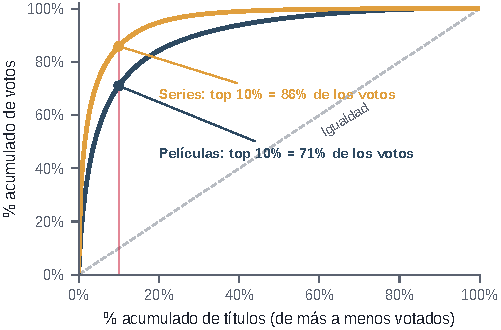
\includegraphics[width=\columnwidth]{p03_concentracion.pdf}
\caption{\textbf{La interacción se concentra en muy pocos títulos.} Curva de Lorenz de los votos por título; la distancia a la diagonal mide la desigualdad.}
\label{fig:lorenz}
\end{figure}
\begin{figure}[!t]
\centering
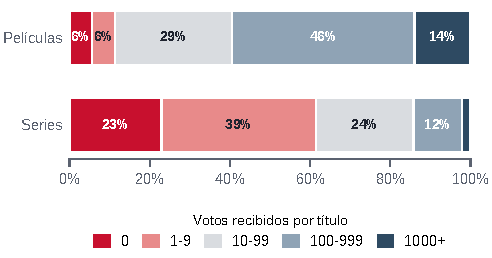
\includegraphics[width=\columnwidth]{p04_visibilidad.pdf}
\caption{\textbf{Seis de cada diez series son prácticamente invisibles.} Distribución de títulos por tramo de votos recibidos.}
\label{fig:visibilidad}
\end{figure}

\hallazgo{El 10\,\% de los títulos más votados concentra el 71\,\% de los votos en películas y el 86\,\% en series (Fig.~\ref{fig:lorenz}). En series, el 22,9\,\% no tiene ningún voto y otro 38,6\,\% tiene entre 1 y 9: el 61,6\,\% es prácticamente invisible. En películas esa proporción es 11,4\,\% (Fig.~\ref{fig:visibilidad}).}

\implica{La plataforma depende de pocos éxitos, y el resto del catálogo casi no aporta a la retención. Un recomendador basado solo en popularidad refuerza este patrón.}

\subsection{P1: la interacción está desalineada con la oferta}
\begin{figure*}[!t]
\centering
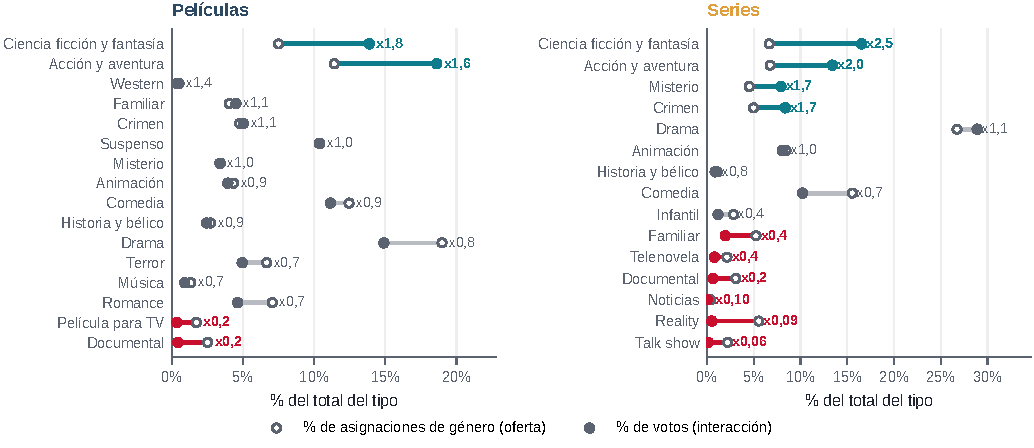
\includegraphics[width=\textwidth]{p01_oferta_interaccion.pdf}
\caption{\textbf{Ciencia ficción y acción generan hasta 2,5 veces más interacción que su peso en la oferta; talk show, reality y noticias casi no generan interacción.} Participación de cada género en la oferta (círculo blanco, \% de asignaciones título-género) y en la interacción (círculo relleno, \% de votos). La etiqueta es el índice de tracción. Petróleo: 1,5 o más; rojo: 0,4 o menos; gris: contexto.}
\label{fig:traccion}
\end{figure*}

\hallazgo{En series, ciencia ficción y fantasía reúne el 6,7\,\% de las asignaciones de género y el 16,5\,\% de los votos (tracción 2,5). Le siguen acción y aventura (1,98), misterio (1,75) y crimen (1,68). Contado por títulos, el 12,2\,\% de las series tiene ese género y concentra el 41\,\% de sus votos. En el otro extremo están talk show (0,06), reality (0,09), noticias (0,10) y documental (0,21): el 14\,\% de las series lleva alguno de los tres primeros y recibe solo el 1,6\,\% de los votos. En películas lideran ciencia ficción y fantasía (1,85) y acción y aventura (1,63); documental (0,17) y películas para TV (0,20) quedan al final. Drama, el género con más títulos, rinde bajo su peso en películas (0,78) (Fig.~\ref{fig:traccion}).}

\implica{Hay espacio para reasignar presupuesto de adquisición hacia géneros con alta tracción. Advertencia: reality y talk show pueden consumirse sin que el público los califique en TMDB; su baja tracción debe confirmarse con datos propios de reproducción antes de desinvertir.}

\subsection{P2: hay contenido bien evaluado que no se descubre}
\begin{figure*}[!t]
\centering
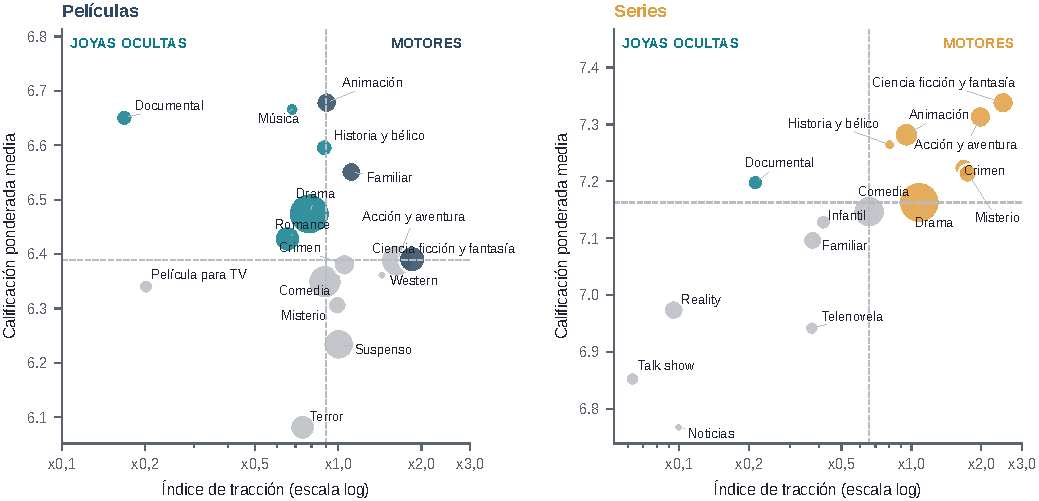
\includegraphics[width=\textwidth]{p02_matriz.pdf}
\caption{\textbf{Documental, música e historia: bien evaluados, pero poco descubiertos.} Matriz calidad vs.\ interacción por género; tamaño = n.º de títulos; líneas punteadas = medianas de los géneros .}
\label{fig:matriz}
\end{figure*}

\hallazgo{Con las medianas como umbral, los \emph{motores} (alta calidad, alta tracción) en series son ciencia ficción y fantasía, acción y aventura, animación, crimen, misterio, historia y bélico, y drama (este último justo en el umbral). En películas lo son animación, familiar y ciencia ficción y fantasía. Las \emph{joyas ocultas} (alta calidad, baja tracción) más marcadas son documental, música e historia y bélico en películas: el 54\,\% de los documentales tiene nota 7 o más, frente al 26\,\% del total de películas. En series, la joya oculta es documental. Drama y romance (películas) también caen en ese cuadrante, pero cerca del umbral de calidad. Terror tiene la calificación más baja y además baja tracción (0,74); suspenso tiene tracción proporcional (1,00) y calidad bajo la mediana (Fig.~\ref{fig:matriz}).}

\implica{Las joyas ocultas son contenido ya disponible, valorado por quien lo ve y poco expuesto: es el insumo más barato para mejorar la experiencia mediante recomendación.}

\subsection{P6: popularidad y calidad son dimensiones distintas}
\begin{figure}[!t]
\centering
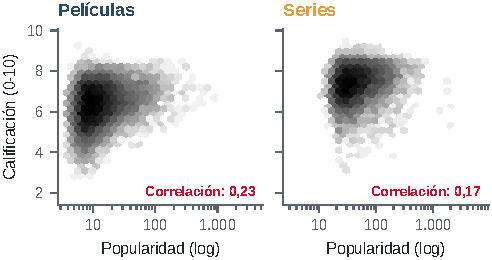
\includegraphics[width=\columnwidth]{p07_popularidad.pdf}
\caption{\textbf{Ser popular no es lo mismo que ser bien evaluado.} Popularidad vs.\ calificación en títulos con 10 o más votos (hexbin; tono más oscuro = más títulos).}
\label{fig:popularidad}
\end{figure}

\hallazgo{La relación entre popularidad y calificación es débil: la correlación es de solo 0,23 en películas y 0,17 en series (Fig.~\ref{fig:popularidad}). Muchos títulos populares tienen notas medias y muchos títulos muy bien evaluados son poco populares.}

\implica{Si la recomendación privilegia la popularidad, refuerza la concentración y oculta calidad. Conviene combinar popularidad con calificación ponderada.}

\subsection{P4: idioma original y calidad percibida}
\begin{figure*}[!t]
\centering
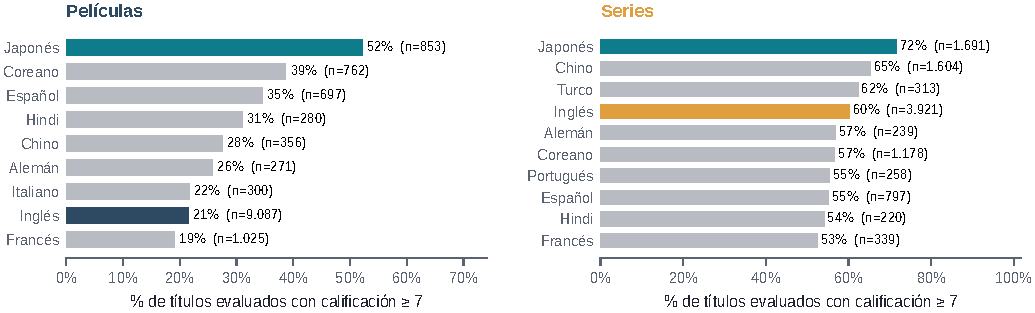
\includegraphics[width=\textwidth]{p05_idiomas.pdf}
\caption{\textbf{El contenido japonés es el mejor evaluado; el inglés domina en volumen, no en calidad.} \% de títulos con nota 7 o más por idioma original (idiomas con 200 o más títulos evaluados). Petróleo = máximo; azul/ámbar = inglés como referencia.}
\label{fig:idiomas}
\end{figure*}

\hallazgo{Entre los idiomas con 200 o más títulos evaluados, el japonés tiene la mayor proporción de títulos bien evaluados: 52\,\% en películas y 72\,\% en series. En películas, coreano (39\,\%) y español (35\,\%) superan ampliamente al inglés (21\,\%), que reúne el 60\,\% de las películas evaluadas y el 88\,\% de sus votos (Fig.~\ref{fig:idiomas}). En series, el coreano (57\,\%) queda \emph{bajo} el inglés (60\,\%). La Tabla~\ref{tab:robustez} muestra que el liderazgo japonés en películas se mantiene con cualquier umbral de votos, mientras que en series su posición depende del umbral (cuarto con 1 o 10 votos mínimos, segundo con 50). Además, el 56\,\% de las películas y el 77\,\% de las series japonesas son animación: el efecto es principalmente anime.}

\begin{table}[!t]
\caption{¿Cambia el resultado si exigimos más votos? Tres idiomas con mayor \% de títulos con nota 7 o más (idiomas con 100 o más títulos)}
\label{tab:robustez}
\centering\footnotesize
\begin{tabularx}{\columnwidth}{@{}P{0.9cm}LL@{}}
\toprule
Votos mín. & Películas & Series\\
\midrule
1 & Japonés 52\,\%, portugués 41\,\%, coreano 39\,\% & Cantonés 82\,\%, tailandés 78\,\%, ruso 73\,\% (japonés 72\,\%, 4.º)\\
10 & Japonés 54\,\%, coreano 48\,\%, portugués 38\,\% & Español 84\,\%, turco 80\,\%, chino 79\,\% (japonés 77\,\%, 4.º)\\
50 & Japonés 59\,\%, coreano 58\,\%, español 37\,\% & Coreano 97\,\%, japonés 94\,\%, español 93\,\%\\
\bottomrule
\end{tabularx}
\end{table}

\implica{El anime japonés es una apuesta de diferenciación robusta en ambos tipos. La producción coreana está respaldada en películas; en series, la evidencia es mixta.}

\subsection{P5: evolución de la calidad percibida}
\begin{figure}[!t]
\centering
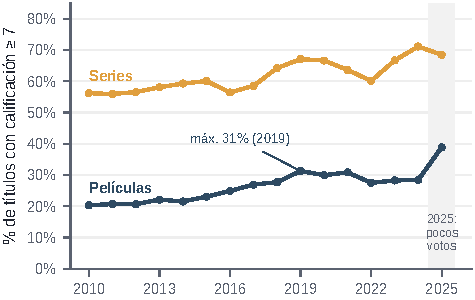
\includegraphics[width=\columnwidth]{p06_tendencia.pdf}
\caption{\textbf{La proporción de títulos bien evaluados tiende a subir desde 2010, con retrocesos.} \% de títulos con nota 7 o más por año de estreno. 2025 se sombrea por tener pocos votos.}
\label{fig:tendencia}
\end{figure}

\hallazgo{Entre 2010 y 2024, la proporción de títulos bien evaluados pasa de 20\,\% a 28\,\% en películas y de 56\,\% a 71\,\% en series. La tendencia es al alza, pero con retrocesos: las películas alcanzan su máximo en 2019 (31\,\%) y retroceden, y las series caen en 2016 y en 2021--2022 (Fig.~\ref{fig:tendencia}). La mediana de votos de las películas baja de 221 (2019) a 61 (2024). Los títulos recientes tienen menos evaluaciones, así que parte del alza puede ser un sesgo de antigüedad. 2025 no se interpreta.}

\implica{La calidad percibida no es el problema del catálogo. El foco debe estar en el descubrimiento.}

\subsection{P7: rentabilidad de las películas}
\begin{figure*}[!t]
\centering
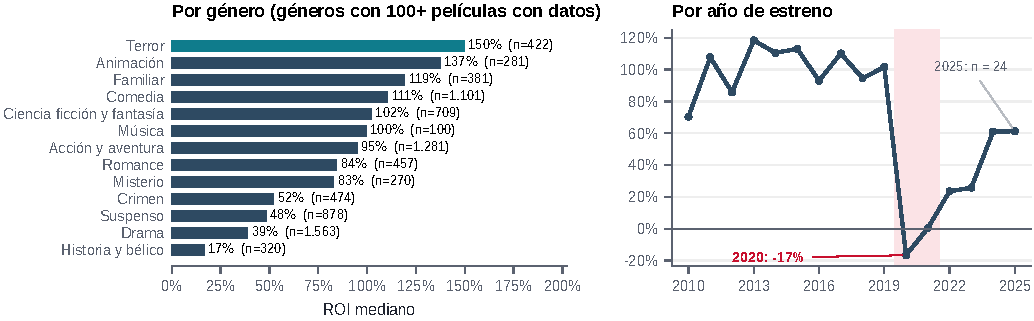
\includegraphics[width=\textwidth]{p08_roi.pdf}
\caption{\textbf{Terror y animación son los géneros más rentables en taquilla; el ROI aún no vuelve a niveles previos a 2020.} ROI mediano de películas con presupuesto y recaudación informados (3.362 películas).}
\label{fig:roi}
\end{figure*}

\hallazgo{Terror (150\,\%), animación (137\,\%) y familiar (119\,\%) tienen el mayor ROI mediano; drama (39\,\%) e historia y bélico (17\,\%), el menor. Terror combina baja calificación con alta rentabilidad por sus presupuestos acotados. El ROI mediano anual promedió cerca de 104\,\% entre 2011 y 2019, cayó a -17\,\% en 2020 y llegó a 61\,\% en 2024. El dato de 2025 se basa en solo 24 películas con recaudación incompleta (Fig.~\ref{fig:roi}).}

\implica{Es relevante solo para coproducciones o licencias con ventana de cine: el ROI mide taquilla, no el valor del título dentro de la plataforma.}

\subsection{P8: origen del contenido}
\begin{figure}[!t]
\centering
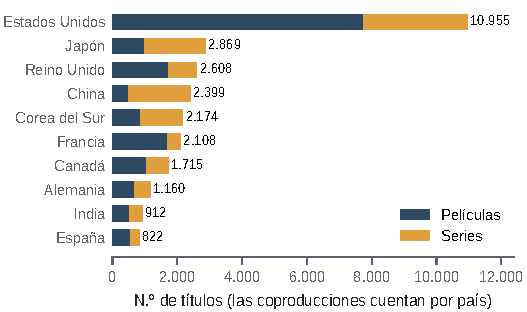
\includegraphics[width=\columnwidth]{p09_paises.pdf}
\caption{\textbf{Estados Unidos domina el origen; Asia pesa más en series que en películas.} Diez países con más títulos (coproducciones cuentan para cada país).}
\label{fig:paises}
\end{figure}

\hallazgo{Estados Unidos participa en 10.955 títulos: el 48,5\,\% de las películas y el 20,0\,\% de las series. Japón (11,8\,\% de las series vs.\ 6,2\,\% de las películas), China (11,9\,\% vs.\ 3,1\,\%) y Corea del Sur (8,1\,\% vs.\ 5,5\,\%) pesan mucho más en series (Fig.~\ref{fig:paises}), lo que coincide con la buena evaluación del contenido japonés.}

% =====================================================================
\section{Diseño y justificación de las representaciones gráficas}
\label{sec:diseno}
\fase{Fase 4: modelado visual}

\subsection{Principios de percepción visual y jerarquía}
\label{sec:percepcion}
\begin{itemize}
\item \textbf{Atención preatentiva:} el color se reserva para el mensaje. El contexto va en gris y solo el dato relevante recibe acento, de modo que el ojo lo detecta antes de leer.
\item \textbf{Gestalt:} \emph{proximidad} (paneles de películas y series lado a lado con ejes comparables), \emph{similitud} (el mismo color significa lo mismo en informe, presentación y dashboard), \emph{cerramiento} (cuadrantes rotulados en la matriz) y \emph{continuidad} (líneas para el tiempo).
\item \textbf{Jerarquía visual:} título-mensaje (en la leyenda del paper y dentro del gráfico en dashboard y presentación), subtítulo con lo que se mide y fuente al pie. El lector recorre la figura en el orden en que debe entenderla.
\item \textbf{Relación dato-tinta:} sin bordes superiores ni derechos, cuadrícula mínima y etiquetas directas en vez de leyendas~\cite{tufte2001}.
\end{itemize}

\subsection{Atributos visuales}
\label{sec:atributos}
Los atributos se asignan según su precisión perceptiva: posición y longitud para los valores que se comparan, y color y tamaño para atributos secundarios~\cite{cleveland1984}. La Tabla~\ref{tab:atributos} detalla el uso de cada uno.

\begin{table}[!t]
\caption{Uso de atributos visuales}
\label{tab:atributos}
\centering\footnotesize
\begin{tabularx}{\columnwidth}{@{}P{1.25cm}LL@{}}
\toprule
Atributo & Uso & Justificación\\
\midrule
Posición & Valores en ejes comunes (Fig.~\ref{fig:lorenz}, \ref{fig:traccion}, \ref{fig:matriz}, \ref{fig:tendencia}) & Atributo más preciso para comparar cantidades\\
Longitud & Barras ordenadas (Fig.~\ref{fig:visibilidad}, \ref{fig:idiomas}, \ref{fig:roi}, \ref{fig:paises}) & Comparación rápida con base común\\
Color (tono) & Azul pizarra = películas, ámbar = series, \textcolor{petroleo}{\textbf{petróleo}} = oportunidad, \textcolor{acento}{\textbf{rojo}} = alerta, gris = contexto & Un solo significado por tono; evita el par verde-rojo, difícil de distinguir con daltonismo\\
Color (luminosidad) & Escala de rojo a azul en visibilidad; gris en hexbin & Orden: más oscuro = más títulos o más votos\\
Tamaño & N.º de títulos por género en la matriz & Tercera variable sin agregar un eje; uso secundario\\
Contraste & Negrita en títulos y en el valor destacado; texto de apoyo en gris & Guía la lectura y separa mensaje de contexto\\
Forma & Círculo vacío (oferta) vs.\ lleno (interacción); línea para el tiempo & Distingue dos medidas en el mismo eje\\
\bottomrule
\end{tabularx}
\end{table}

\subsection{Reducción de la carga cognitiva}
\label{sec:carga}
Para no saturar al lector limitamos cada figura a un mensaje y cada dashboard a seis KPIs. Además, rotulamos directamente en lugar de usar leyendas, ordenamos las barras por valor, usamos escala logarítmica cuando el rango lo exige (tracción de 0,06 a 2,5; popularidad) y aplicamos formato numérico local (coma decimal). También anotamos en el gráfico las advertencias necesarias (2025 con pocos votos, pocos datos), para que el lector no tenga que buscarlas en el texto.

\subsection{Selección de gráficos según la naturaleza de los datos}
\label{sec:seleccion}
La Tabla~\ref{tab:graficos} relaciona cada figura con la estructura de sus datos y la tarea analítica, y registra la alternativa descartada.

\begin{table*}[!t]
\caption{Selección del tipo de gráfico según la naturaleza de los datos y la tarea}
\label{tab:graficos}
\centering\footnotesize
\begin{tabularx}{\textwidth}{@{}P{0.5cm}P{2.9cm}P{3.6cm}P{2.2cm}LP{3.0cm}@{}}
\toprule
Fig. & Tipo de gráfico & Naturaleza de los datos & Tarea & Por qué este gráfico & Alternativa descartada\\
\midrule
\ref{fig:lorenz} & Curva de Lorenz & Distribución de una variable cuantitativa (votos) en 16.000 títulos & Concentración & Estándar para desigualdad; la distancia a la diagonal es la brecha & Pareto de barras: 16.000 barras ilegibles\\
\ref{fig:visibilidad} & Barra apilada 100\,\% & 5 tramos ordenados, 2 categorías & Composición & Tramos ordenados con color secuencial & Torta: los ángulos se comparan peor\\
\ref{fig:traccion} & Mancuernas (dumbbell) & 2 proporciones por categoría nominal & Brecha entre dos medidas & La longitud de la línea es la brecha & Barras agrupadas: duplican elementos\\
\ref{fig:matriz} & Burbujas por cuadrantes & 2 cuantitativas + 1 de tamaño, por categoría & Relación y segmentación & Los cuadrantes traducen el dato a una acción & Tabla: exige comparar mentalmente\\
\ref{fig:popularidad} & Hexbin & 2 cuantitativas, más de 20.000 puntos & Correlación & Evita la sobreposición de puntos & Dispersión simple: saturada\\
\ref{fig:idiomas} & Barras horizontales ordenadas & 1 proporción por categoría nominal con nombres largos & Ranking & Lectura fácil y orden explícito & Mapa: el idioma no es geográfico\\
\ref{fig:tendencia} & Línea temporal & Proporción por año (ordinal temporal) & Tendencia & La continuidad se percibe como evolución & Barras por año: fragmentan la tendencia\\
\ref{fig:roi} & Barras + línea & Mediana por categoría y por año & Ranking y tendencia & Cada panel usa el gráfico de su tarea & Boxplot: menos accesible para la gerencia\\
\ref{fig:paises} & Barras apiladas horizontales & Conteo por país y tipo & Ranking con composición & Total y mezcla en una barra & Mapa coroplético (se usa en el dashboard)\\
\bottomrule
\end{tabularx}
\end{table*}

% =====================================================================
\section{Desarrollo de la narrativa visual (data storytelling)}
\label{sec:narrativa}
\fase{Fase 6: despliegue (comunicación)}

\subsection{Estructura}
La narrativa está dirigida a la audiencia primaria y se presenta en diez minutos. Sigue un arco de tres actos (contexto, conflicto y resolución) que va de la situación a la decisión~\cite{knaflic2015} (Fig.~\ref{fig:arco} y Tabla~\ref{tab:actos}).

\begin{figure}[!t]
\centering
\begin{tikzpicture}[font=\scriptsize]
\draw[-{Stealth[length=4pt]}, grisosc] (0,0) -- (8.3,0) node[above left]{tiempo};
\draw[-{Stealth[length=4pt]}, grisosc] (0,0) -- (0,2.55) node[above right]{tensión};
\draw[line width=1.4pt, acento] plot[smooth, tension=0.6] coordinates {(0.1,0.35) (1.6,0.6) (3.4,1.65) (4.9,2.15) (6.2,1.0) (8.0,0.45)};
\foreach \x/\t/\c in {0.9/{\textbf{1. Contexto}\\catálogo amplio,\\calidad al alza}/pelicula, 3.7/{\textbf{2. Conflicto}\\86\,\% en el top 10\,\%;\\oferta desalineada;\\joyas ocultas}/acento, 6.9/{\textbf{3. Resolución}\\idea central y\\3 decisiones}/petroleo}
  \node[align=center, text=\c, anchor=north] at (\x,-0.12) {\t};
\node[fill=crema, rounded corners=2pt, align=center, inner sep=2pt] at (5.05,2.5) {``No más títulos: que se descubran los correctos''};
\end{tikzpicture}
\caption{Arco narrativo: la tensión crece con la evidencia del problema y se resuelve con decisiones medibles.}
\label{fig:arco}
\end{figure}

\begin{table}[!t]
\caption{Guion de la narrativa y recursos de comunicación}
\label{tab:actos}
\centering\footnotesize
\begin{tabularx}{\columnwidth}{@{}P{1.3cm}LP{1.3cm}P{1.4cm}@{}}
\toprule
Acto & Mensaje & Evidencia & Recurso\\
\midrule
1. Contexto & Catálogo amplio (31.991 títulos, 83 idiomas) cuya calidad percibida no es el problema & Tabla~\ref{tab:kpis}, Fig.~\ref{fig:tendencia} & Oral: situar\\
2. Conflicto & La interacción se concentra en el 10\,\% de los títulos y el 62\,\% de las series es invisible & Fig.~\ref{fig:lorenz}, \ref{fig:visibilidad} & Visual: cifra en grande\\
2. Conflicto & Se ofrece mucho de lo que no genera interacción y se esconde lo que el usuario valora & Fig.~\ref{fig:traccion}, \ref{fig:matriz}, \ref{fig:idiomas} & Visual: énfasis de color\\
3. Resolución & ``No necesitamos más títulos: necesitamos que se descubran los correctos'' & Idea central & Escrito: frase única\\
3. Resolución & Tres decisiones con indicadores y un plan para medir comportamiento real & Tabla~\ref{tab:recomendaciones}, dashboard & Oral + visual: llamado a la acción\\
\bottomrule
\end{tabularx}
\end{table}

\subsection{Integración de recursos orales, escritos y visuales}
\textbf{Visual:} una idea por diapositiva y un gráfico con un solo énfasis de color. Las figuras de la presentación se rediseñan con un panel y texto de al menos 11 pt para la proyección. \textbf{Escrito:} títulos-mensaje y un máximo de dos líneas de apoyo; el detalle queda en este informe y en las notas del orador. \textbf{Oral:} cada integrante narra un acto y explica ``qué significa'' y ``qué hacemos con esto'', sin leer la diapositiva. \textbf{Demostración:} en el acto 3, filtrar el dashboard por \emph{Documental} muestra en vivo una joya oculta: la calificación sube (66\,\% bien evaluados vs.\ 42\,\% del catálogo) y la baja visibilidad también (47\,\% vs.\ 36\,\%).

\subsection{Plan de exposición}
La presentación dura diez minutos y cada integrante narra un bloque del arco (Tabla~\ref{tab:exposicion}). Como la nota es individual y puede haber preguntas cruzadas, los tres integrantes preparan todo el contenido con la guía de defensa.

\begin{table}[!t]
\caption{Plan de exposición y recursos por bloque}
\label{tab:exposicion}
\centering\footnotesize
\begin{tabularx}{\columnwidth}{@{}P{1.35cm}P{1.05cm}P{0.8cm}L@{}}
\toprule
Integrante & Diap. & Tiempo & Contenido y recurso dominante\\
\midrule
Claudio Aro & 1--5 & 3:00 & Acto 1: problema, audiencias, estrategia, CRISP-DM y datos. Oral para situar; tarjetas visuales\\
Guillermo Cerda & 6--11 & 3:40 & Acto 2: hallazgos y justificación técnica de los gráficos. Visual: cifra grande y un énfasis de color\\
Manuel Díaz & 12--16 & 3:00 & Acto 3: idea central, dashboard, recomendaciones, evaluación y cierre. Escrito (frase única) y llamado a la acción\\
\bottomrule
\end{tabularx}
\end{table}

\subsection{Coherencia entre visualizaciones, audiencia y propósito}
\label{sec:coherencia}
La Tabla~\ref{tab:coherencia} verifica que cada pieza visual responde una pregunta de negocio, llega a la audiencia correcta y sostiene una decisión. Así se evitan gráficos ``decorativos'' sin propósito.

\begin{table*}[!t]
\caption{Matriz de coherencia: visualización, pregunta, audiencia, propósito y decisión}
\label{tab:coherencia}
\centering\footnotesize
\begin{tabularx}{\textwidth}{@{}P{2.4cm}P{0.6cm}P{3.3cm}P{2.4cm}L@{}}
\toprule
Visualización & Preg. & Audiencia principal & Propósito & Decisión que habilita\\
\midrule
Lorenz y visibilidad (Fig.~\ref{fig:lorenz}, \ref{fig:visibilidad}) & P3 & Gerencia general; Producto/UX & Persuadir (conflicto) & Priorizar el descubrimiento sobre la compra de más títulos\\
Tracción (Fig.~\ref{fig:traccion}) & P1 & Gerencia general; Contenidos & Persuadir (conflicto) & Reasignar presupuesto de adquisición por género\\
Matriz (Fig.~\ref{fig:matriz}) & P2 & Producto/UX; Contenidos & Persuadir e informar & Crear filas de ``joyas ocultas''\\
Popularidad vs.\ calificación (Fig.~\ref{fig:popularidad}) & P6 & Producto/UX; Analítica & Informar & Combinar popularidad con calidad en el ranking\\
Idiomas y países (Fig.~\ref{fig:idiomas}, \ref{fig:paises}) & P4, P8 & Contenidos; estrategia internacional & Informar & Ampliar anime y contenido japonés\\
Tendencia (Fig.~\ref{fig:tendencia}) & P5 & Gerencia general & Contextualizar & Descartar la calidad como problema principal\\
ROI (Fig.~\ref{fig:roi}) & P7 & Finanzas / producción & Informar & Géneros para coproducción con ventana de cine\\
Dashboard (Fig.~\ref{fig:dash1}--\ref{fig:dash4}) & P1--P8 & Gerencias operativas; Analítica & Habilitar la exploración & Consultas propias sin depender de analítica\\
\bottomrule
\end{tabularx}
\end{table*}

% =====================================================================
\section{Diseño e implementación del dashboard interactivo}
\label{sec:dashboard}
\fase{Fase 6: despliegue (herramienta)}

\subsection{Tecnología y componentes}
El dashboard se implementó con Streamlit (interfaz y navegación) y Plotly (gráficos interactivos), reutilizando los módulos \texttt{src/} del análisis. Se ejecuta con \texttt{streamlit run dashboard/app.py}. La Tabla~\ref{tab:dashboard} resume sus componentes.

\begin{table}[!t]
\caption{Componentes del dashboard}
\label{tab:dashboard}
\centering\footnotesize
\begin{tabularx}{\columnwidth}{@{}P{1.55cm}L@{}}
\toprule
Componente & Implementación\\
\midrule
KPIs (6) & Títulos, votos, calificación ponderada, \% bien evaluados, \% baja visibilidad y concentración top 10\,\%. Al filtrar, muestran la diferencia contra el catálogo completo (con color invertido cuando subir es malo).\\
Filtros globales (5) & Tipo, rango de años, géneros, idioma original y votos mínimos; botón para restablecer; aplican a todas las páginas.\\
Navegación (6 páginas) & Resumen ejecutivo; géneros; idiomas y origen; tendencias; explorador de títulos; metodología y glosario.\\
Interacción & Tooltips; selección por clic o lazo en la matriz que despliega los títulos del género; selector de indicador en tendencias; mapa con zoom; búsqueda por título, director o reparto; interruptor ``solo joyas ocultas''.\\
Exportación & Descarga en CSV de la selección filtrada.\\
Ayuda y estados & Íconos de ayuda en cada KPI, recuadro ``cómo leer'' por página, mensajes calculados sobre la selección y aviso cuando un filtro deja la vista sin datos.\\
\bottomrule
\end{tabularx}
\end{table}

\begin{figure*}[!t]
\centering
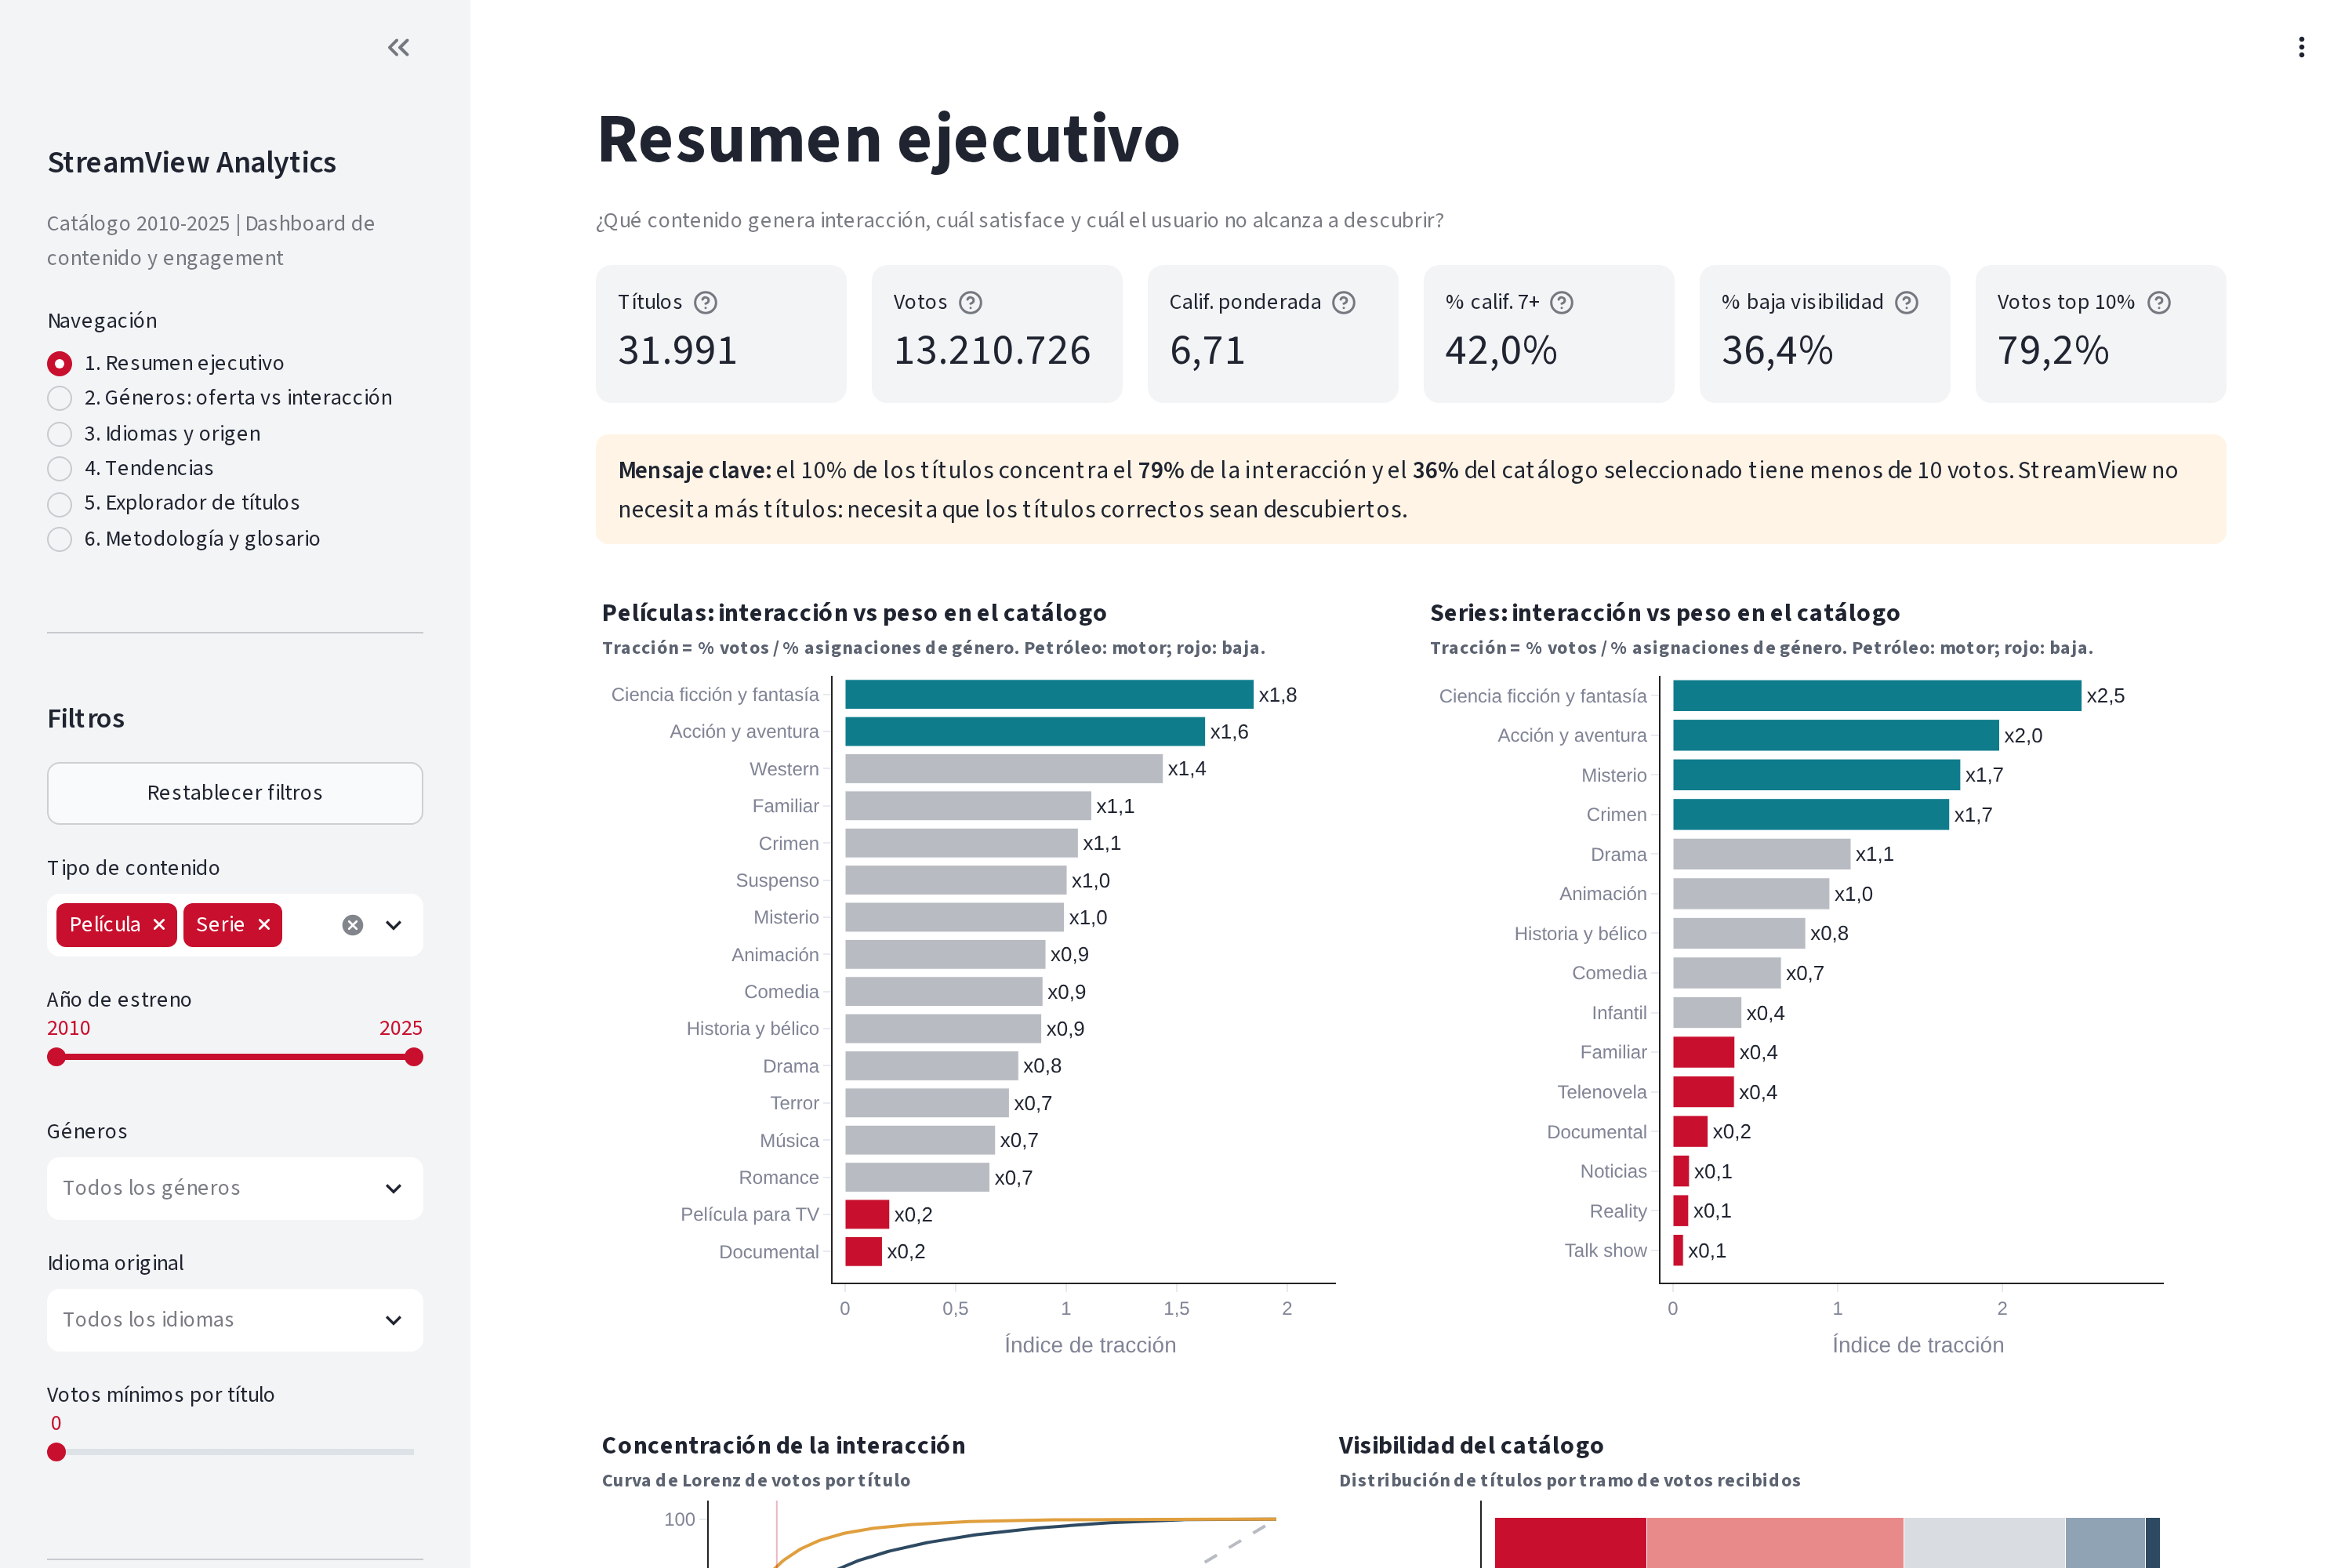
\includegraphics[width=0.49\textwidth]{dash_p1.png}\hfill
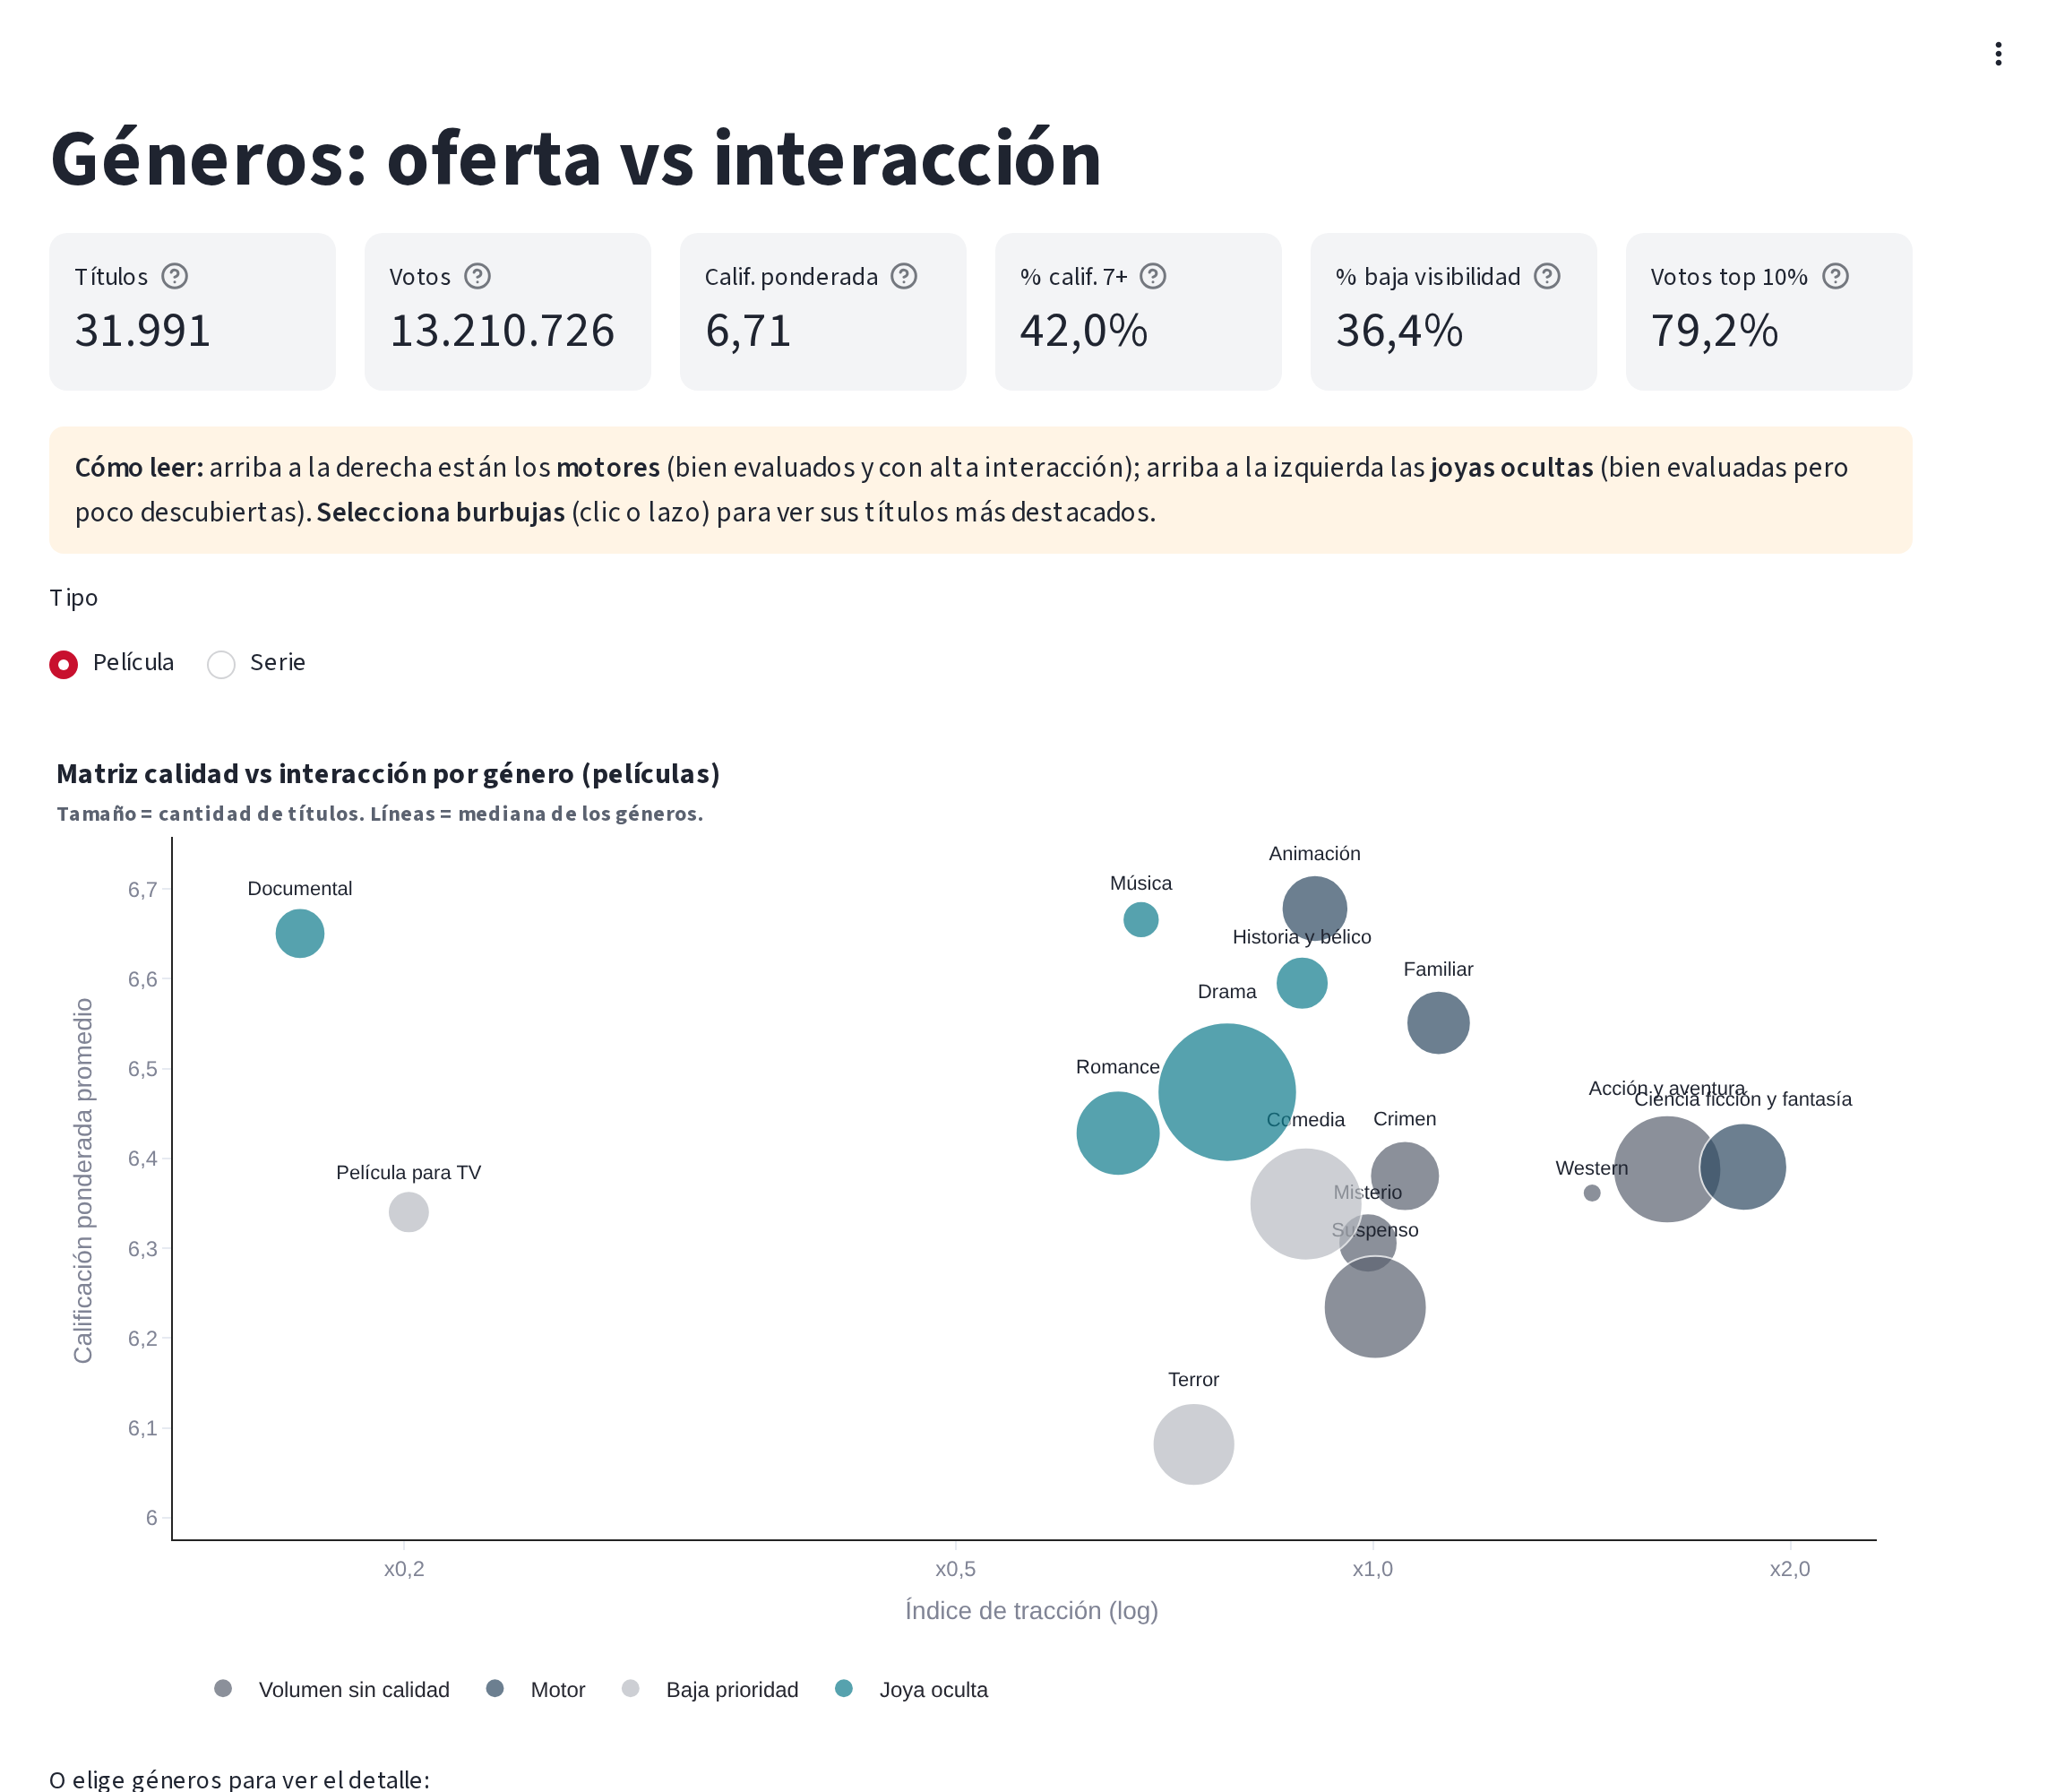
\includegraphics[width=0.49\textwidth]{dash_p2_crop.png}
\caption{Dashboard. Izquierda: página 1 (resumen ejecutivo) con filtros globales, seis KPIs, mensaje clave y tracción por género. Derecha: página 2, matriz interactiva calidad vs.\ interacción; seleccionar burbujas despliega los títulos mejor evaluados del género.}
\label{fig:dash1}
\end{figure*}
\begin{figure*}[!t]
\centering
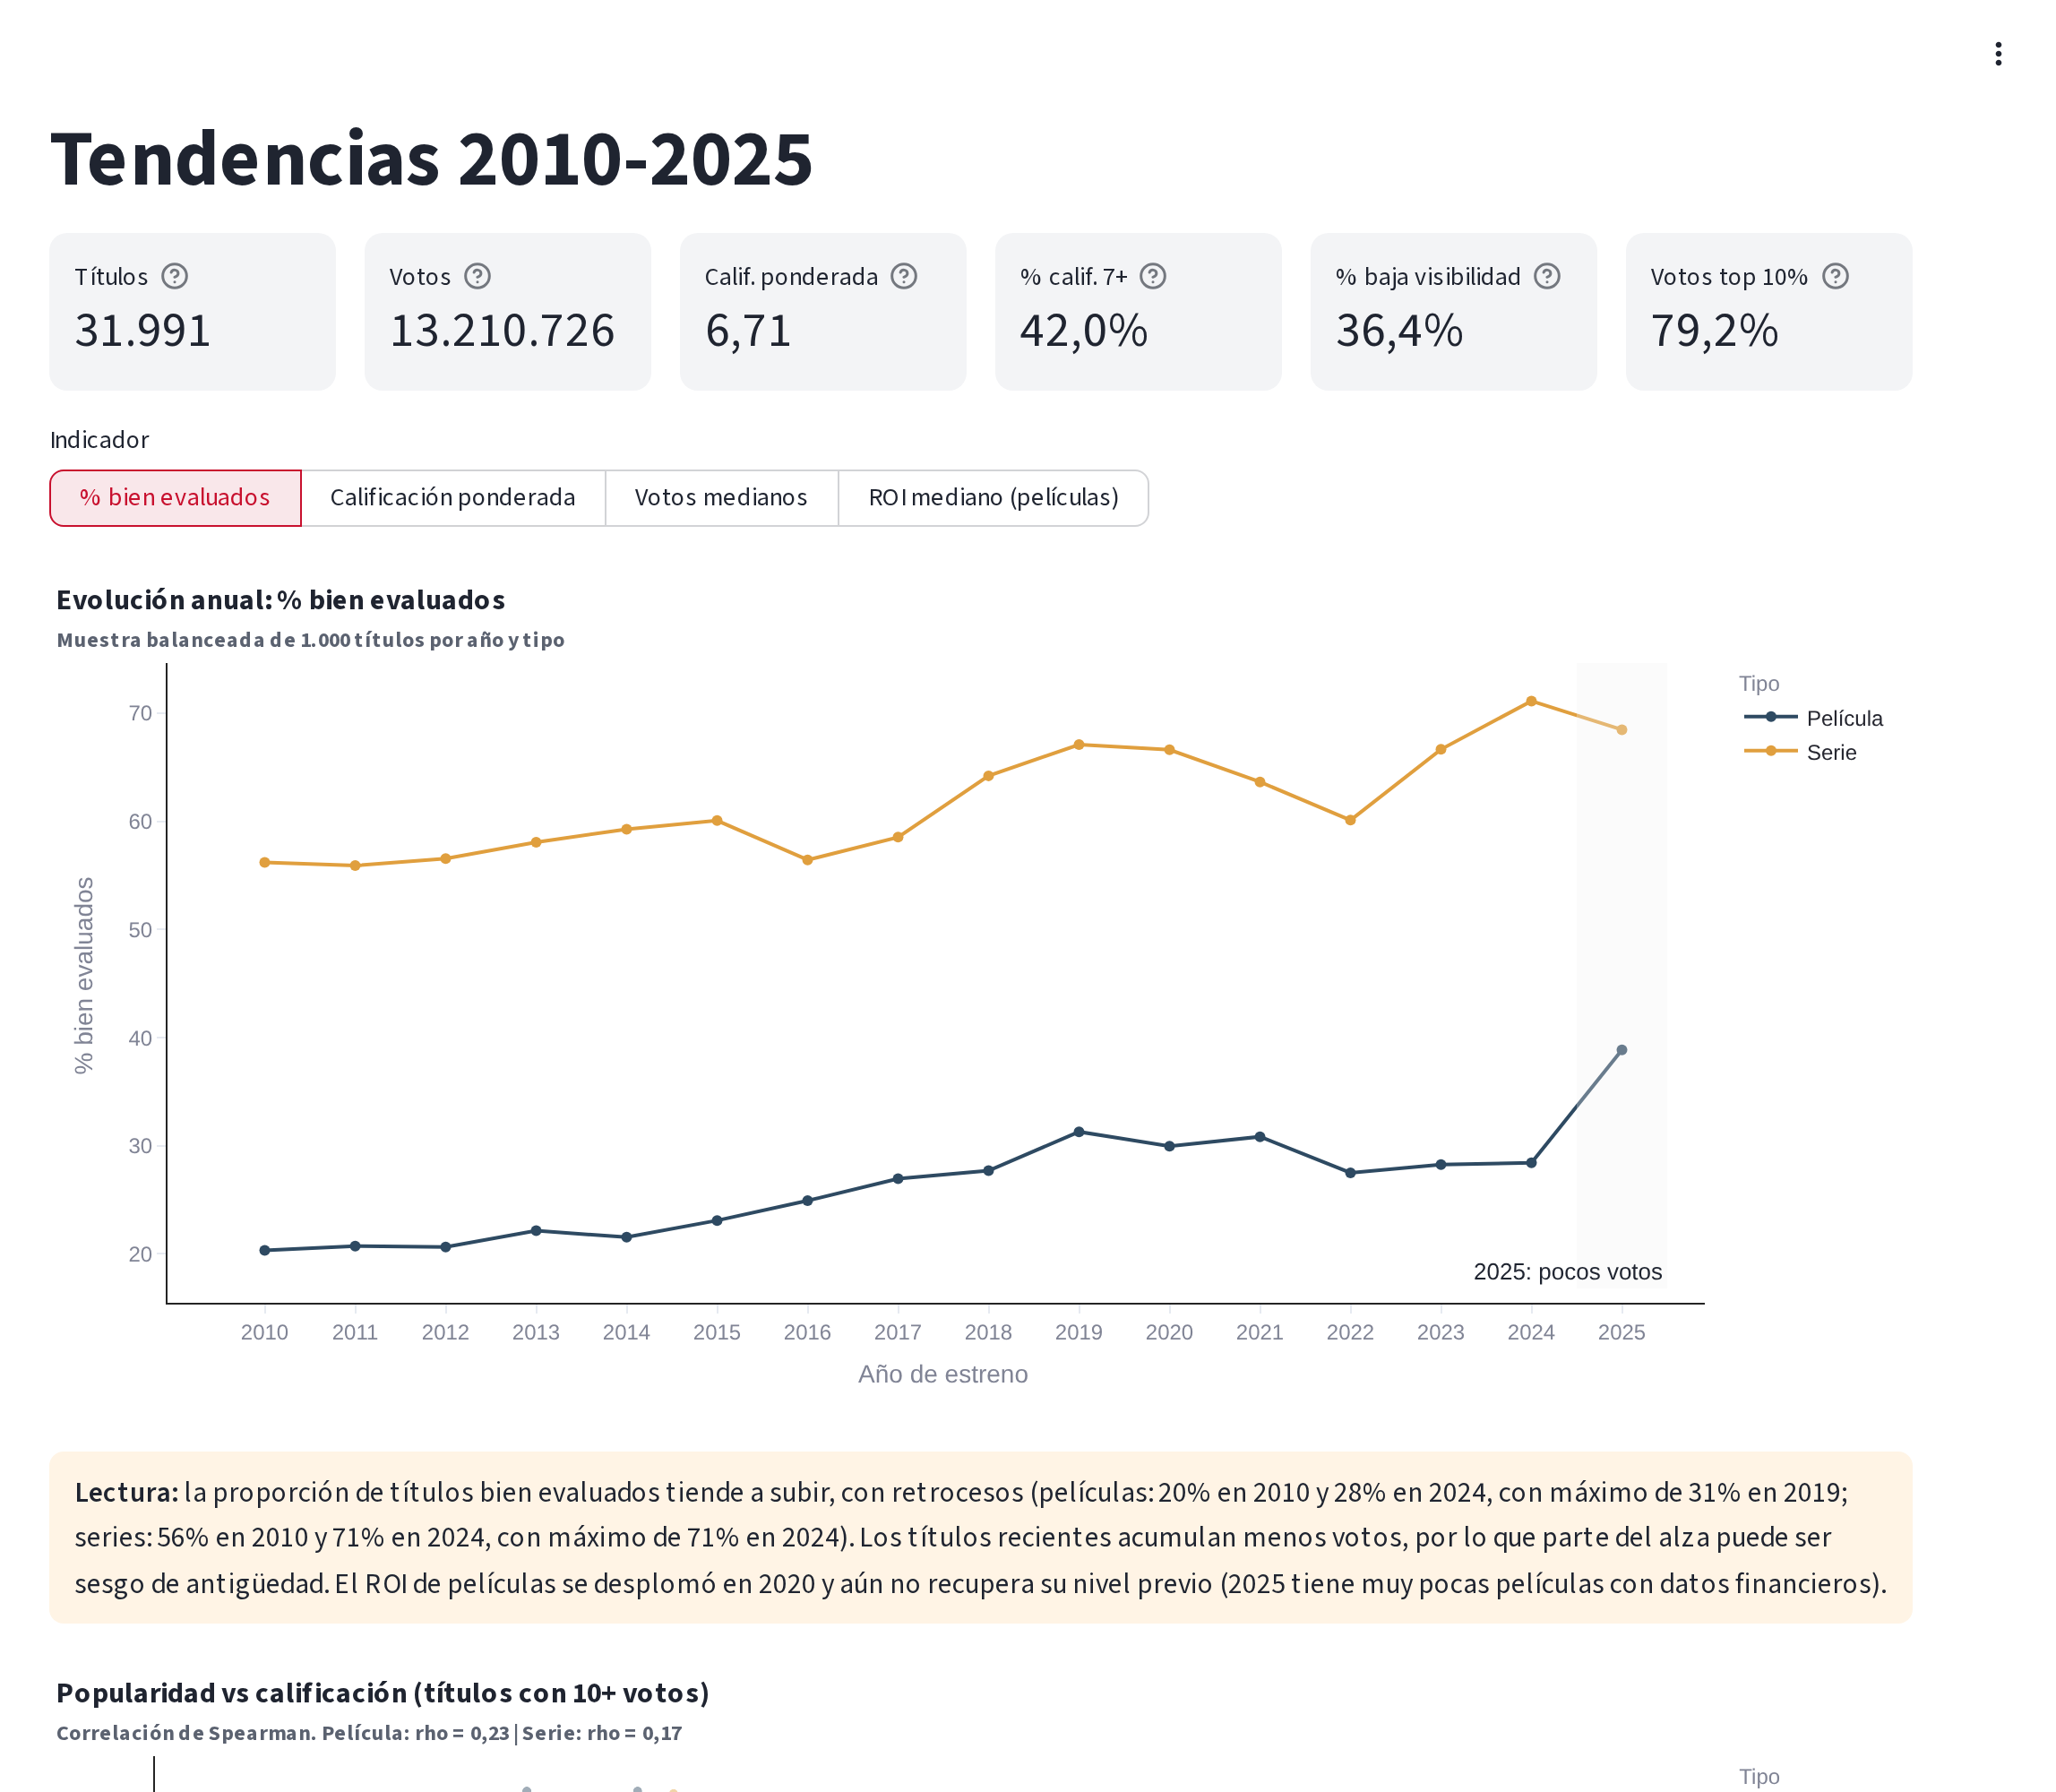
\includegraphics[width=0.49\textwidth]{dash_p4_crop.png}\hfill
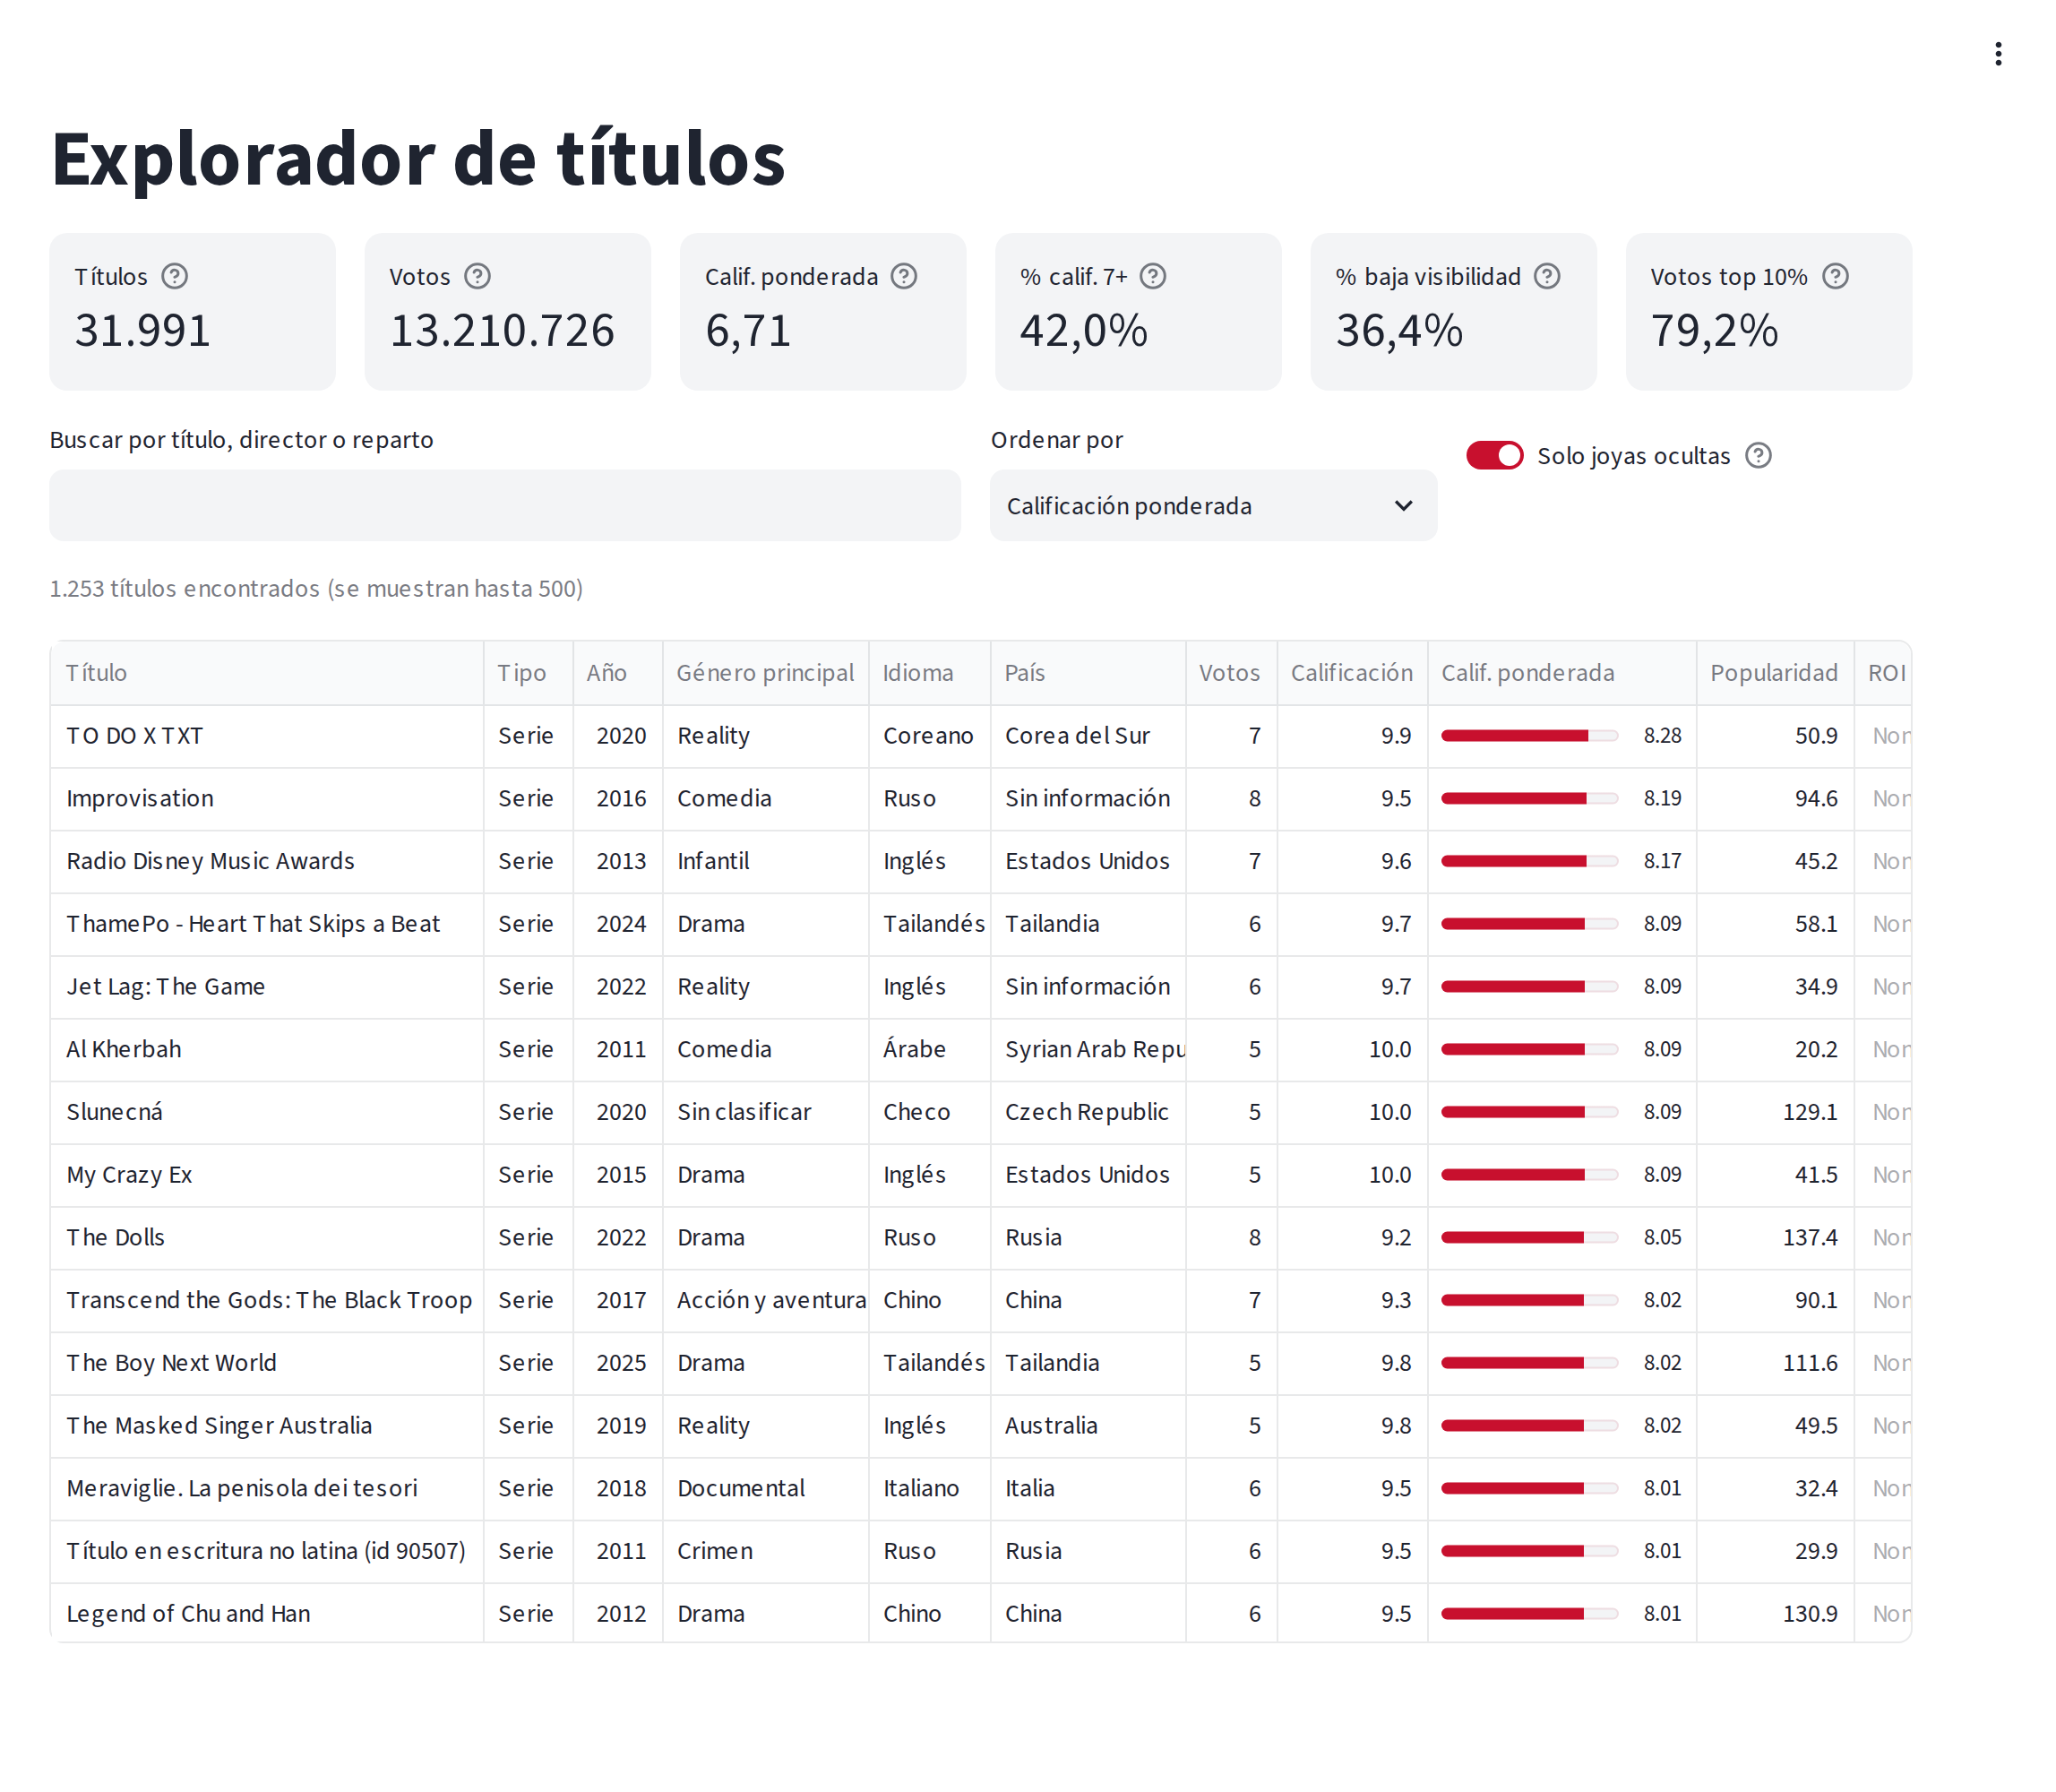
\includegraphics[width=0.49\textwidth]{dash_p5_crop.png}
\caption{Dashboard. Izquierda: página 4 (tendencias), con selector de indicador y lectura calculada sobre la selección. Derecha: página 5 (explorador), con búsqueda, orden y filtro ``solo joyas ocultas'' (1.253 títulos en el catálogo completo).}
\label{fig:dash4}
\end{figure*}

\subsection{Decisiones de diseño}
\begin{itemize}
\item \textbf{Lectura en Z y de lo general a lo particular:} KPIs arriba, mensaje clave, gráficos de síntesis y, al final, tablas de detalle~\cite{few2006}.
\item \textbf{Un solo lugar de control:} los filtros de la barra lateral aplican a todas las páginas y mantienen la coherencia entre vistas.
\item \textbf{Consistencia cromática} con el informe y la presentación: el usuario aprende los colores una sola vez.
\item \textbf{Seis KPIs como máximo}, para no superar la capacidad de la memoria de trabajo.
\item \textbf{Textos dinámicos:} los mensajes de la página de tendencias se calculan sobre la selección y no se escriben como cifras fijas, de modo que el texto nunca contradice al gráfico.
\end{itemize}

\begin{table*}[!t]
\caption{Recomendaciones, evidencia, responsable e indicador de seguimiento}
\label{tab:recomendaciones}
\centering\footnotesize
\begin{tabularx}{\textwidth}{@{}P{0.3cm}LP{2.6cm}P{1.9cm}P{5.0cm}@{}}
\toprule
N.º & Recomendación & Evidencia (fuerza) & Responsable & Indicador y meta\\
\midrule
1 & Crear filas de ``joyas ocultas'' y una cuota de exposición para títulos bien evaluados con poca interacción; combinar popularidad y calificación ponderada en el ranking del recomendador. & Fig.~\ref{fig:lorenz}, \ref{fig:visibilidad}, \ref{fig:matriz}, \ref{fig:popularidad} (alta: patrón en ambos tipos) & Producto / UX & \% del catálogo con al menos una reproducción en 90 días y \% de reproducciones del top 10\,\%: medir la línea base y reducir la concentración en 12 meses, validado con prueba A/B (proxy actual: 86\,\% y 62\,\% en series).\\
2 & Priorizar la adquisición de ciencia ficción y fantasía y acción y aventura (y misterio y crimen en series); revisar la inversión en talk show, reality y noticias después de confirmar su bajo consumo con datos propios. & Fig.~\ref{fig:traccion} (media: proxy TMDB) & Contenidos y adquisiciones & Tracción calculada con reproducciones de las nuevas adquisiciones de al menos 1,0 (proxy actual en votos: 1,6--2,5 en géneros priorizados).\\
3 & Ampliar y destacar el anime y el contenido japonés en ambos tipos, y el coreano en películas. & Fig.~\ref{fig:idiomas}, \ref{fig:paises}; Tabla~\ref{tab:robustez} (alta en películas, media en series) & Contenidos / Marketing & Participación del contenido japonés en reproducciones y calificación interna de los títulos incorporados.\\
4 & En coproducciones con ventana de cine, favorecer géneros de alto ROI (terror, animación, familiar) y controlar presupuestos en drama e historia. & Fig.~\ref{fig:roi} (media: solo taquilla) & Finanzas / Producción & ROI mediano de coproducciones frente a la referencia prepandemia (cerca de 100\,\%).\\
5 & Instrumentar datos de reproducción, abandono, suscripción y dispositivo, e integrarlos al dashboard. & Secc.~\ref{sec:evaluacion} (alta: brecha estructural) & Analítica / TI & Página de retención y churn operativa en 6 meses.\\
\bottomrule
\end{tabularx}
\end{table*}

% =====================================================================
\section{Evaluación crítica de la solución}
\label{sec:evaluacion}
\fase{Fase 5: evaluación}

\subsection{Fortalezas}
\begin{itemize}
\item \textbf{Una sola fuente de verdad:} datos y métricas centralizados en \texttt{src/}; las cifras del dashboard, las figuras, la presentación y este informe son idénticas y reproducibles con tres comandos.
\item \textbf{Indicadores comparables} entre películas y series: taxonomía unificada, calificación ponderada e índice de tracción.
\item \textbf{Afirmaciones verificadas:} cada hallazgo se recalculó y los que dependen de un supuesto se presentan con su prueba de robustez (Tabla~\ref{tab:robustez}).
\item \textbf{Narrativa con una idea central} y un dashboard con exploración real (selección en gráficos, búsqueda, exportación).
\end{itemize}

\subsection{Limitaciones}
\begin{itemize}
\item \textbf{Proxies externos:} votos, calificación y popularidad provienen de TMDB, no de los suscriptores de StreamView. Miden a quien califica, que no representa a toda la base, y no permiten medir retención ni abandono.
\item \textbf{Sin datos de comportamiento:} no hay reproducciones, minutos vistos, suscripciones ni dispositivos, fuentes que el caso sí menciona.
\item \textbf{Muestra por cuota:} 1.000 títulos por año y tipo, con un criterio de selección no documentado; no permite analizar crecimiento ni generalizar al catálogo completo.
\item \textbf{Sesgo de antigüedad:} los títulos recientes acumulan menos votos; afecta la tendencia (Fig.~\ref{fig:tendencia}) y el ROI de 2025.
\item \textbf{Series con pocos votos:} en series, la calificación ponderada corrige poco porque la referencia es de solo 9 votos; las joyas ocultas de series tienen una mediana de 4 votos, así que son candidatas, no evidencia firme.
\item \textbf{Datos financieros parciales:} solo el 21\,\% de las películas tiene ROI válido, y el ROI mide taquilla, no el valor dentro de la plataforma.
\end{itemize}

\subsection{Oportunidades de mejora}
\begin{itemize}
\item Incorporar eventos de uso (reproducción, abandono, sesión) y de suscripción para construir KPIs de retención y \emph{churn}, y recalcular la tracción con reproducciones.
\item Exigir más votos de referencia en series para que la calificación ponderada sea más estable.
\item Publicar el dashboard en un servidor corporativo con actualización automática y control de acceso por rol; traducir los nombres de países que aún aparecen en inglés.
\item Validar el diseño con pruebas de usabilidad con cada gerencia (tiempo en responder una pregunta) y evaluar las recomendaciones con pruebas A/B.
\end{itemize}

\subsection{Decisiones de diseño reconsideradas}
Descartamos la calificación simple por género porque los títulos con pocos votos generaban promedios engañosos, y la reemplazamos por la ponderada. Descartamos también un índice de tracción común para películas y series, porque las películas concentran el 87\,\% de los votos y ocultaban a las series. El gráfico de idiomas del dashboard pasó de barras agrupadas a puntos para reducir la carga visual. Detectamos que el rojo se usaba a la vez para alertas y para resultados positivos, así que adoptamos un color de significado único con petróleo para las oportunidades. Por último, precisamos que la tracción se calcula sobre asignaciones título-género y no sobre títulos, y reemplazamos los textos con cifras fijas del dashboard por textos calculados.

% =====================================================================
\section{Conclusiones y recomendaciones}
\label{sec:conclusiones}
\fase{Fases 5 y 6: evaluación y despliegue (decisión)}

\subsection{Conclusiones}
\begin{enumerate}
\item \textbf{El problema principal es de descubrimiento, no de oferta.} El 10\,\% de los títulos concentra el 71\,\% (películas) y el 86\,\% (series) de los votos, y el 62\,\% de las series tiene menos de 10 votos.
\item \textbf{La oferta está desalineada con la interacción.} Ciencia ficción y fantasía y acción y aventura rinden hasta 2,5 veces su peso; talk show, reality y noticias, menos de 0,1.
\item \textbf{Hay calidad escondida.} Documental, música e historia (películas) y documental (series) están bien evaluados y son poco descubiertos, y popularidad y calidad apenas se relacionan (0,17--0,23).
\item \textbf{El anime japonés es la oportunidad de calidad más robusta}; el contenido coreano y el español destacan en películas.
\item \textbf{La calidad percibida no es el problema:} tiende a subir entre 2010 y 2024, con retrocesos y un posible sesgo de antigüedad.
\end{enumerate}

\subsection{Recomendaciones}
La Tabla~\ref{tab:recomendaciones} vincula cada recomendación con su evidencia, la fuerza de esa evidencia, su responsable y su indicador. Como los votos provienen de una comunidad externa, las metas se definen sobre datos propios de reproducción. Las cifras actuales se informan solo como línea base aproximada.



En síntesis, la mejor inversión inmediata de StreamView no es comprar más contenido, sino hacer visible el valor que ya tiene y medir, con datos propios, si eso aumenta la permanencia de sus suscriptores.

% =====================================================================
\appendices
\section{Trazabilidad con las pautas de evaluación}
\noindent\begin{minipage}{\columnwidth}\centering\footnotesize
\textbf{EP1 --- Encargo}\\[2pt]
\begin{tabularx}{\columnwidth}{@{}P{3.1cm}L@{}}
\toprule
Indicador & Dónde se evidencia\\
\midrule
IE4 Percepción visual y jerarquía (14\,\%) & Secc.~\ref{sec:percepcion}; títulos-mensaje en todas las figuras; Fig.~\ref{fig:dash1}\\
IE5 Atributos visuales (16\,\%) & Secc.~\ref{sec:atributos}, Tabla~\ref{tab:atributos}\\
IE6 Comprensión y carga cognitiva (20\,\%) & Secc.~\ref{sec:carga}; anotaciones en Fig.~\ref{fig:tendencia}, \ref{fig:roi}\\
IE7 Tipo de gráfico según los datos (12\,\%) & Secc.~\ref{sec:seleccion}, Tabla~\ref{tab:graficos}\\
IE9 Coherencia visual--audiencia--propósito (20\,\%) & Secc.~\ref{sec:audiencia}, Tabla~\ref{tab:coherencia}\\
IE10 Narrativa visual (18\,\%) & Secc.~\ref{sec:narrativa}, Fig.~\ref{fig:arco}, Tabla~\ref{tab:actos}\\
\bottomrule
\end{tabularx}
\end{minipage}\par\medskip
\noindent\begin{minipage}{\columnwidth}\centering\footnotesize
\textbf{EP2 --- Presentación}\\[2pt]
\begin{tabularx}{\columnwidth}{@{}P{3.1cm}L@{}}
\toprule
Indicador & Dónde se evidencia (informe y presentación)\\
\midrule
IE1 Audiencia y contexto (12\,\%) & Secc.~\ref{sec:audiencia}, Tabla~\ref{tab:audiencias}; diapositiva 2\\
IE2 Propósito y problema de negocio (16\,\%) & Secc.~\ref{sec:problema} y \ref{sec:audiencia}-B; diapositiva 2\\
IE3 Estrategia de comunicación (22\,\%) & Secc.~\ref{sec:estrategia}, Tabla~\ref{tab:estrategia}; diapositiva 3\\
IE8 Justificación técnica de las representaciones (18\,\%) & Secc.~\ref{sec:diseno}, Tablas~\ref{tab:atributos} y \ref{tab:graficos}; diapositiva 11 y pie de cada gráfico\\
IE11 Recursos orales, escritos y visuales (14\,\%) & Secc.~\ref{sec:narrativa}-B y -C, Tablas~\ref{tab:actos} y \ref{tab:exposicion}; notas del orador\\
IE12 Conclusiones con evidencia (18\,\%) & Secc.~\ref{sec:conclusiones}, Tabla~\ref{tab:recomendaciones}; diapositiva 14\\
\bottomrule
\end{tabularx}\\[6pt]
\textbf{Metodología}: CRISP-DM, Secc.~\ref{sec:metodologia}, Fig.~\ref{fig:crisp}, Tabla~\ref{tab:crisp}; diapositiva 4.
\end{minipage}\par\medskip

\section{Estructura y ejecución del proyecto}
Carpetas: \texttt{data/raw} (fuentes), \texttt{data/processed} (tablas integradas), \texttt{src/} (\texttt{config}, \texttt{preparacion}, \texttt{metricas}, \texttt{graficos}, \texttt{graficos\_paper}), \texttt{notebooks/} (01 integración y 02 análisis, ejecutados), \texttt{dashboard/app.py}, \texttt{images/} y \texttt{docs/} (este informe, presentación, guía de defensa y \texttt{VALIDACION.md}). Ejecución: \texttt{pip install -r requirements.txt}; \texttt{python -m src.preparacion}; \texttt{python -m src.graficos\_paper}; \texttt{streamlit run dashboard/app.py}.

% =====================================================================
\begin{thebibliography}{99}
\footnotesize
\bibitem{tmdb} The Movie Database (TMDB), ``API documentation.'' [En línea]. Disponible: https://developer.themoviedb.org
\bibitem{knaflic2015} C.~N. Knaflic, \emph{Storytelling with Data: A Data Visualization Guide for Business Professionals}. Hoboken, NJ, USA: Wiley, 2015.
\bibitem{tufte2001} E.~R. Tufte, \emph{The Visual Display of Quantitative Information}, 2.ª ed. Cheshire, CT, USA: Graphics Press, 2001.
\bibitem{cleveland1984} W.~S. Cleveland y R.~McGill, ``Graphical perception: Theory, experimentation, and application to the development of graphical methods,'' \emph{J. Amer. Statist. Assoc.}, vol.~79, no.~387, pp.~531--554, 1984.
\bibitem{chapman2000} P.~Chapman \emph{et al.}, \emph{CRISP-DM 1.0: Step-by-step data mining guide}. SPSS Inc., 2000.
\bibitem{few2006} S.~Few, \emph{Information Dashboard Design: The Effective Visual Communication of Data}. Sebastopol, CA, USA: O'Reilly, 2006.
\end{thebibliography}

\end{document}
